\documentclass[11pt]{article}

\usepackage[margin=1in]{geometry}
\usepackage{amsmath, amssymb}
\usepackage{graphicx}
\usepackage{subcaption}
\usepackage{booktabs}
\usepackage{placeins}
\usepackage[colorlinks=true,linkcolor=black,urlcolor=blue,citecolor=black]{hyperref}
\usepackage[capitalise,noabbrev]{cleveref}

\title{\textbf{High Performance Parallel Computing \\ Homework 3: Parallel LU Factorization}}
\author{Liam Pohlmann, Alex Shaffer}
\date{\today}

\begin{document}

\maketitle

%The figures below come from the sweeps run on the \texttt{eng-instruction} partition (AMD EPYC 7713 nodes, up to 128 MPI ranks on one node, one rank per core). The test matrix is $A=S+NI$ with $N=n+1$, factored as the augmented system $[A\,|\,b]$ with $b=A\mathbf{1}$, without pivoting. Throughout, ``GFLOPS'' uses $\tfrac{2}{3}n^3$ operations, and ``efficiency'' is the GFLOPS per rank of a run divided by the GFLOPS of the 1-rank run with the same $n$ (or the same $n^2/PQ$) and block size. $PQ$ is the number of ranks, and the dotted line in every efficiency plot marks 80\%.

% =====================================================================
For this homework assignment we consider factoring the augmented linear system $[A \ | \ \underbar{b}] = LU$ with $\underbar{b} = A\underbar{1}$.
We lay the matrix out on a 2D $P \times Q$ block-cyclic processor grid with block size $b$.
We consider two different, but related, approaches to solving this problem in a parallel manner. 

\begin{itemize}
    \item unblocked (BLAS1)
    \item blocked (BLAS3)
\end{itemize}


\section*{Question 1: unblocked (BLAS1) factorization}



\subsection{Correctness}
We began by verifying that our facorization is correct. For small matrices we looked at different P and Q and measured the residual norm.
\cref{tab:lu-correctness} shows that we reach near machine precision as expected for a correct factorization using a well conditioned matrix such as the one from the homework. 
\begin{table}[htbp]
  \centering
  \begin{tabular}{rrr ccc}
    \toprule
    $P$ & $Q$ & Ranks &
    $\dfrac{\|A - LU\|_F}{\|A\|_F}$ &
    $\dfrac{\|b - A\hat{x}\|_\infty}{\|A\|_\infty \|\hat{x}\|_\infty}$ &
    $\|\hat{x} - \mathbf{1}\|_\infty$ \\
    \midrule
    1 & 1 &  1 & $4.97\times10^{-16}$ & $3.50\times10^{-15}$ & $3.77\times10^{-15}$ \\
    1 & 2 &  2 & $4.97\times10^{-16}$ & $3.50\times10^{-15}$ & $3.77\times10^{-15}$ \\
    2 & 1 &  2 & $4.97\times10^{-16}$ & $3.50\times10^{-15}$ & $3.77\times10^{-15}$ \\
    1 & 4 &  4 & $4.97\times10^{-16}$ & $3.50\times10^{-15}$ & $3.77\times10^{-15}$ \\
    4 & 1 &  4 & $4.97\times10^{-16}$ & $3.50\times10^{-15}$ & $3.77\times10^{-15}$ \\
    2 & 2 &  4 & $4.97\times10^{-16}$ & $3.50\times10^{-15}$ & $3.77\times10^{-15}$ \\
    2 & 3 &  6 & $4.97\times10^{-16}$ & $3.50\times10^{-15}$ & $3.77\times10^{-15}$ \\
    3 & 2 &  6 & $4.97\times10^{-16}$ & $3.50\times10^{-15}$ & $3.77\times10^{-15}$ \\
    2 & 4 &  8 & $4.97\times10^{-16}$ & $3.50\times10^{-15}$ & $3.77\times10^{-15}$ \\
    4 & 2 &  8 & $4.97\times10^{-16}$ & $3.50\times10^{-15}$ & $3.77\times10^{-15}$ \\
    3 & 4 & 12 & $4.97\times10^{-16}$ & $3.50\times10^{-15}$ & $3.77\times10^{-15}$ \\
    4 & 3 & 12 & $4.97\times10^{-16}$ & $3.50\times10^{-15}$ & $3.77\times10^{-15}$ \\
    4 & 4 & 16 & $4.97\times10^{-16}$ & $3.50\times10^{-15}$ & $3.77\times10^{-15}$ \\
    \bottomrule
  \end{tabular}
  \caption{Correctness of the parallel unblocked LU factorization for
    $m = 503$, $n = m+1$ (augmented $[A \mid b]$ with $b = A\mathbf{1}$),
    block size $n_b = 1$, on a range of $P \times Q$ process grids.
    $\hat{x}$ is obtained by back substitution with the computed $U$.}
    \label{tab:lu-correctness}
\end{table}

\subsection{Strong and weak scaling}

We then moved on to strong and weak scaling pictured in \cref{fig:q1_strong} and \cref{fig:q1_weak} respectivly. 
In the strong scaling plots we look at a few differnt linear system sizes $n$ and plot both the total time and the speed up factor.
We see what we expect here. The total time goes down as the number of ranks increases, and for a while it goes down very near the ideal.
Eventaully, when $PQ$ becomes large relative to the problem size the speedup stagnates. This is particularly visible for the largest case.
In that case it seems that cache size and memory contention play a role. 
In the case of the weak scaling, we again see the expoected trend. We keep the local memory per rank constant, but for the LU factorization the FLOPS per rank grows.
This means that the total time increases as we weak scale.
The time doessn't quite grow like the expected $O(\sqrt(PQ))$ but deviating from that is expected as communication starts to play a bigger role at larger $PQ$.
The efficiency panel for the weak scaling shows curves that stay efficient at small ranks but begin to fall more precipitously at higher ones.
All cases drop below 80 \% parallel efficiency between 4 and 16 ranks.


\begin{figure}[htbp]
    \centering
    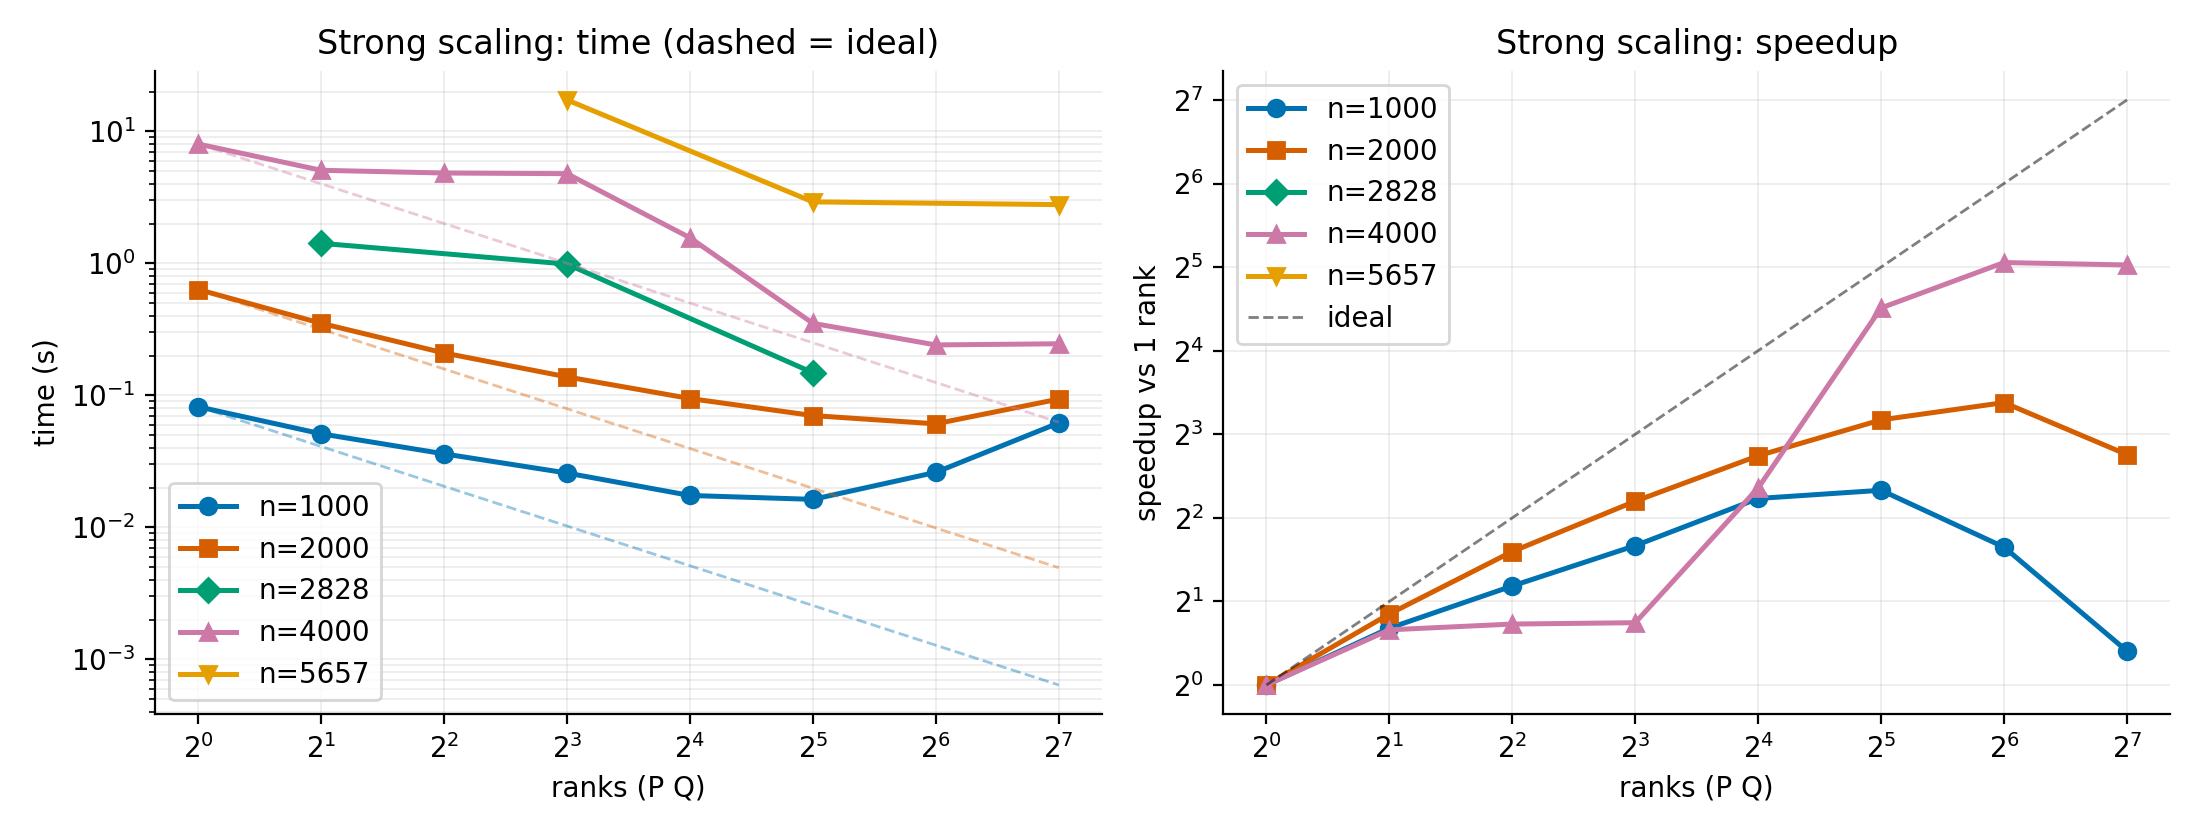
\includegraphics[width=\textwidth]{figs/strong.png}
    \caption{Q1 strong scaling for $n=4000$, $8000$ and $16000$ on 1 to 128 ranks, log--log. Left: time to factor; dashed lines are ideal $1/(PQ)$ scaling from the 1-rank run. Right: speedup over the 1-rank run; dashed line is ideal.}
    \label{fig:q1_strong}
\end{figure}

\begin{figure}[htbp]
    \centering
    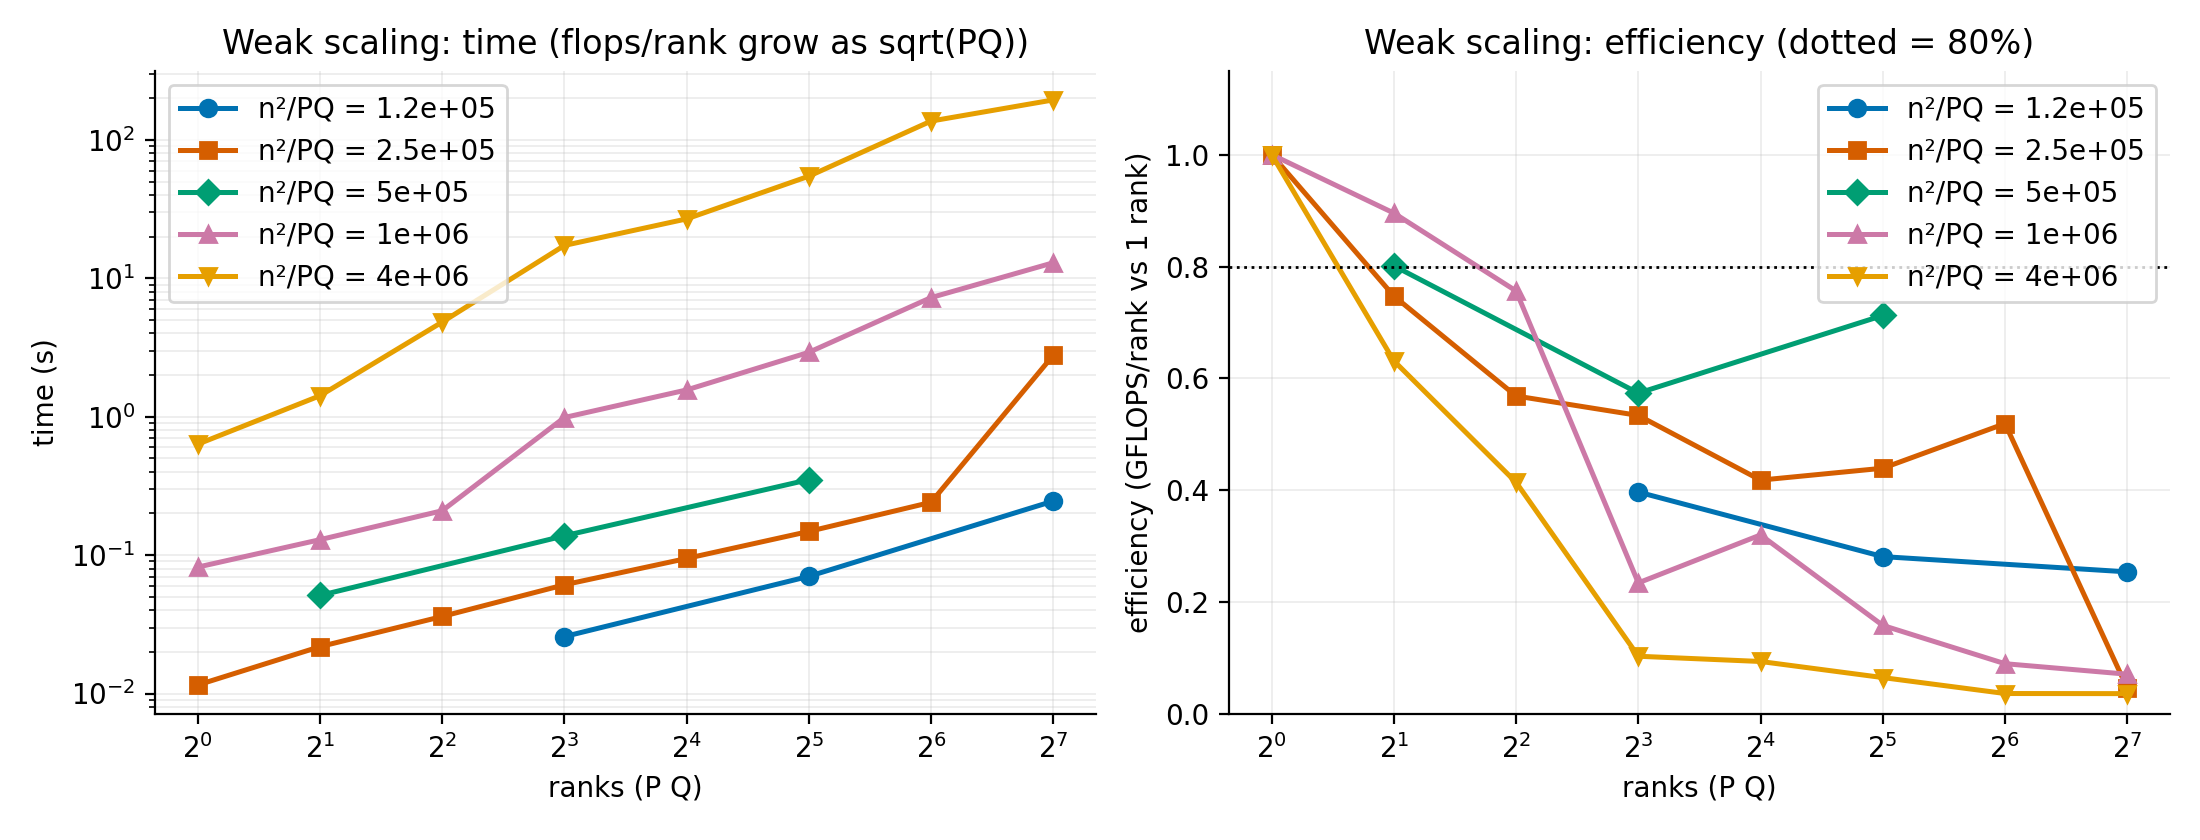
\includegraphics[width=\textwidth]{figs/weak.png}
    \caption{Q1 weak scaling for $n^2/(PQ)=10^6$, $4\times10^6$ and $1.6\times10^7$ doubles per rank on 1 to 128 ranks. Left: time to factor (log scale); the flops per rank grow as $\sqrt{PQ}$. Right: efficiency, GFLOPS per rank divided by that of the 1-rank run with the same $n^2/(PQ)$; dotted line is 80\%.}
    \label{fig:q1_weak}
\end{figure}

\FloatBarrier

\subsection{Local memory footprint for 80\% efficiency}
Next, we looked at the relationship between local memory footprint and parallel efficiency.
\cref{fig:q1_eff_footprint} and \cref{fig:q1_eff_total} show the efficiency versus the local footprint and efficiency versus the total matrix size respectivly.
In \cref{fig:q1_eff_footprint} we see that for the rank counts that hit the 80\% parallel efficiency that local footprint was in the range of $10^6 - 10^7$ doubles per rank.

\begin{figure}[htbp]
    \centering
    \begin{subfigure}[t]{0.49\textwidth}
        \centering
        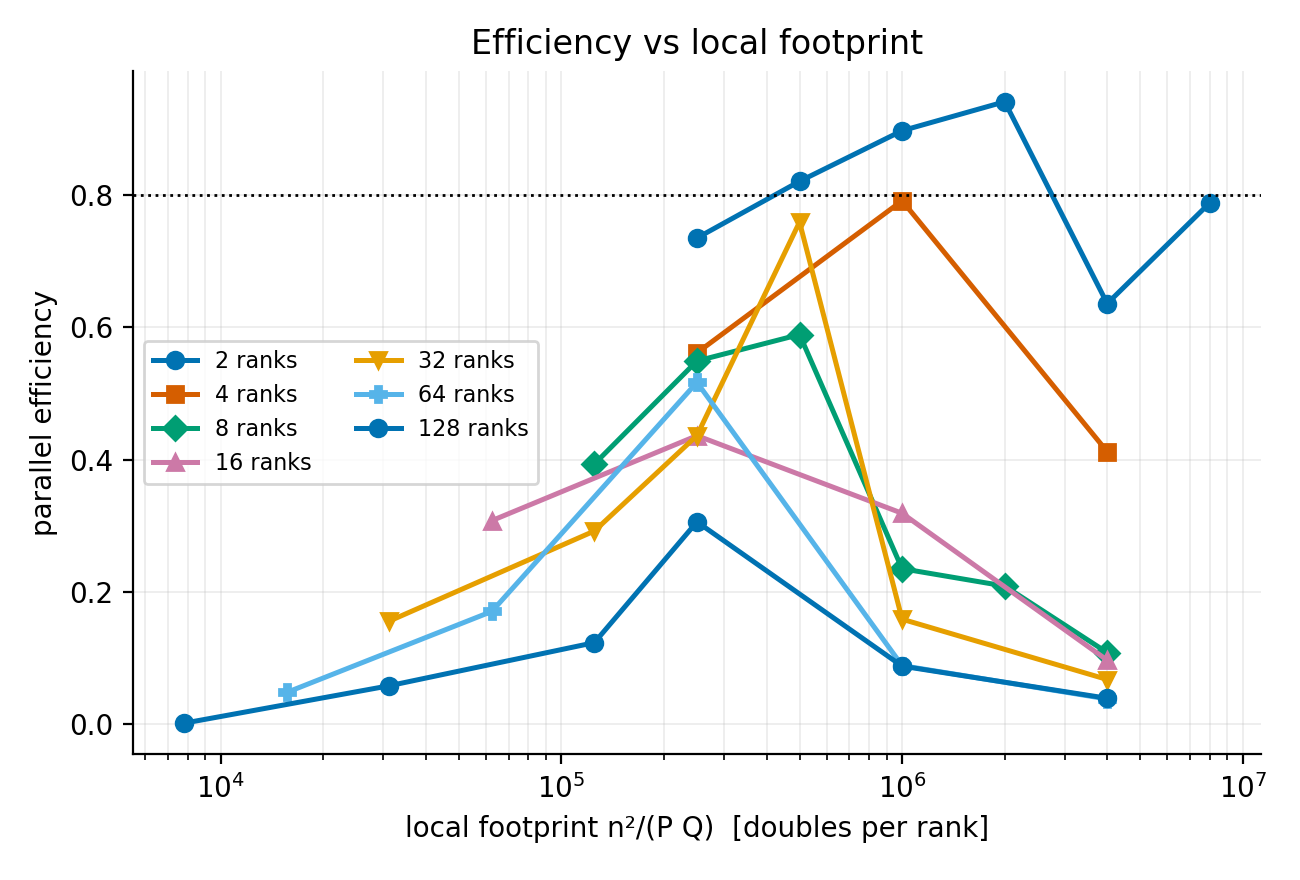
\includegraphics[width=\textwidth]{figs/efficiency_footprint.png}
        \caption{Against the local footprint $n^2/(PQ)$ (doubles per rank).}
        \label{fig:q1_eff_footprint}
    \end{subfigure}\hfill
    \begin{subfigure}[t]{0.49\textwidth}
        \centering
        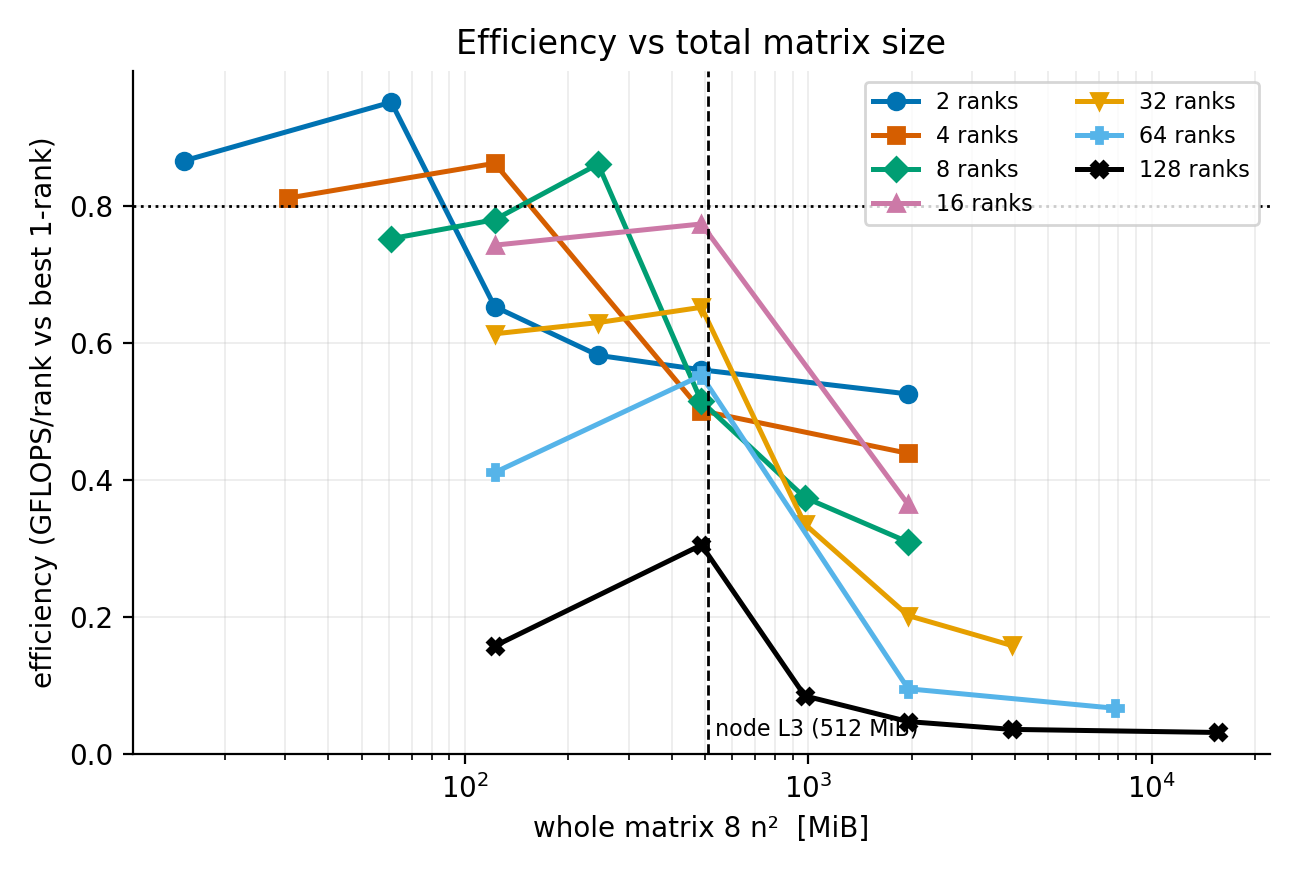
\includegraphics[width=\textwidth]{figs/efficiency_total.png}
        \caption{Against the size of the whole matrix, $8n^2$ bytes; the dashed line is the node's combined L3 cache (512\,MiB).}
        \label{fig:q1_eff_total}
    \end{subfigure}
    \caption{Q1 efficiency of every strong- and weak-scaling run with more than one rank, one curve per rank count. Here efficiency is GFLOPS per rank divided by the best 1-rank GFLOPS (8.50), so that strong and weak runs share one baseline. Dotted line: 80\%.}
    \label{fig:q1_eff}
\end{figure}

\FloatBarrier
\subsection{Observed GFLOPS}
We also looked at the GFLOPS of the runs. \cref{fig:q1_gflops} shows total GFLOPS and GFLOPS per rank versus the total number of ranks. 
We see that initially the total GLFOPS increase, but then begin to decrease past around $16$ ranks for these runs.
This is consistent with were we have seen the performance fall off in the earlier runs. It seems that memory and communication become more expensive there.
The GFLOPS per rank decreases steadly in each case until it drops more quickly, again around $16$ ranks.
In this figure we see a maximum total GFLOPS of around 300.
\begin{figure}[htbp]
    \centering
    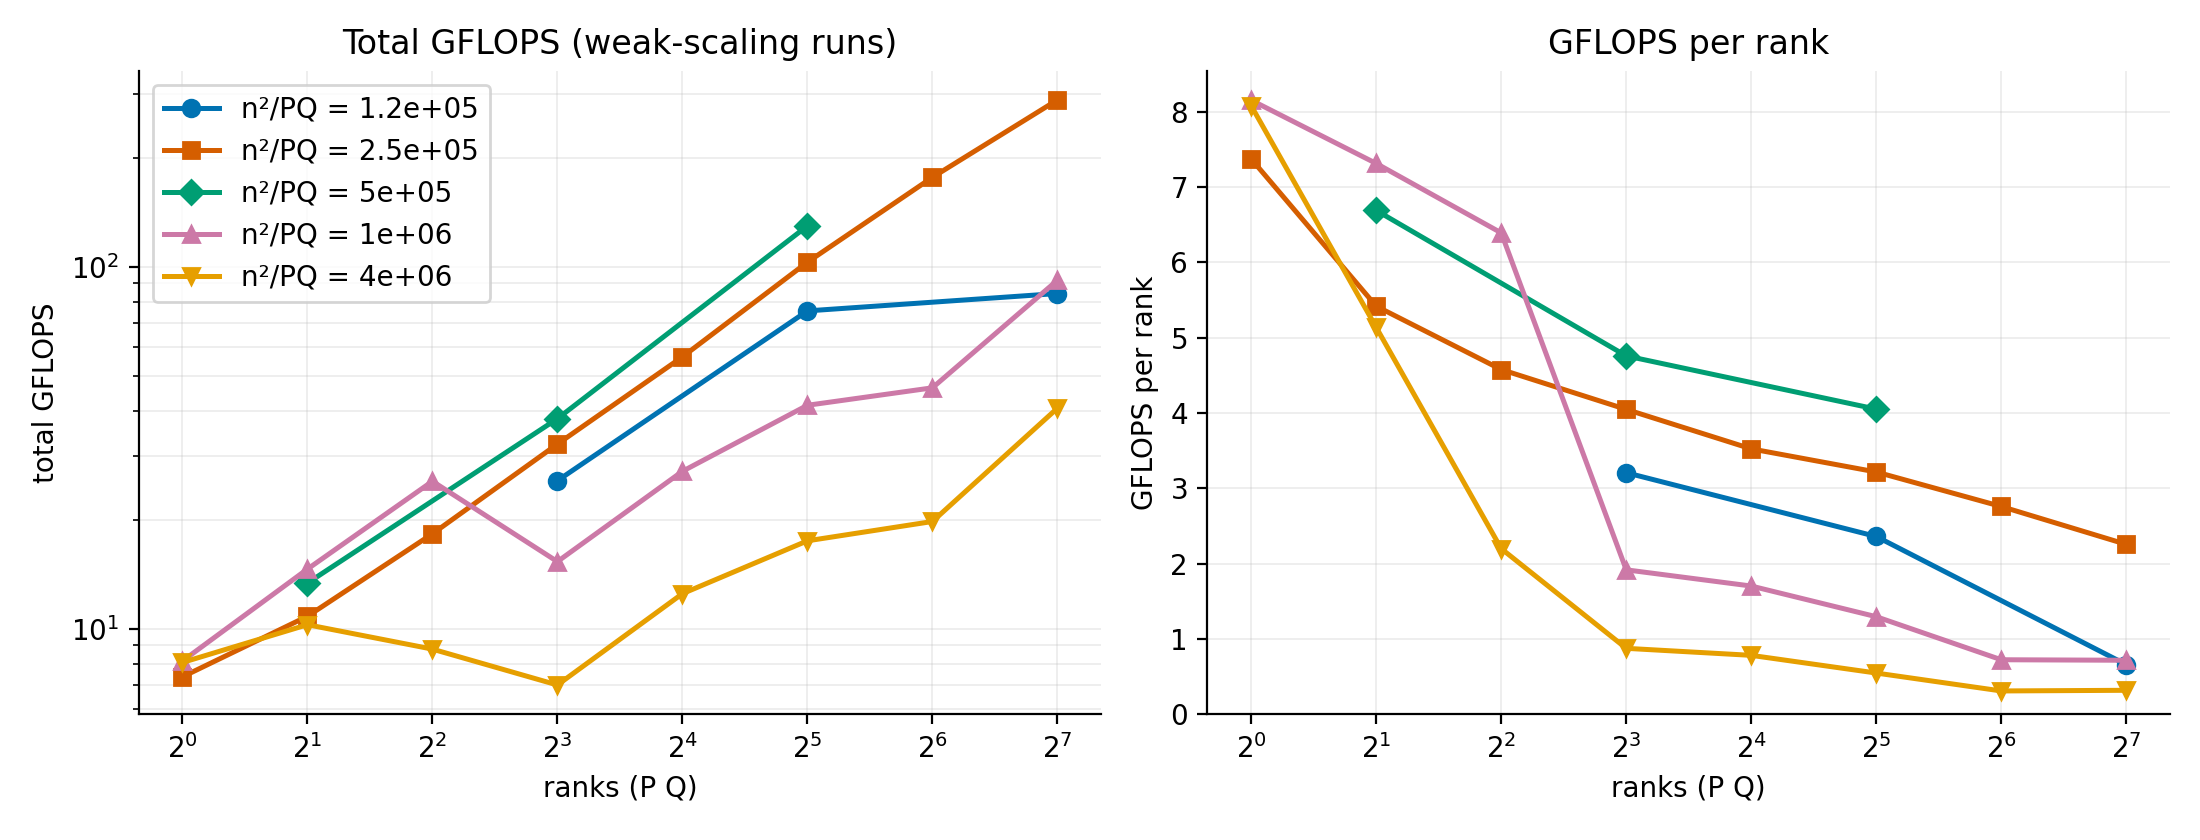
\includegraphics[width=\textwidth]{figs/gflops.png}
    \caption{Q1 GFLOPS of the weak-scaling runs against the number of ranks, one curve per $n^2/(PQ)$. Left: total GFLOPS (log scale). Right: GFLOPS per rank.}
    \label{fig:q1_gflops}
\end{figure}

% =====================================================================
\FloatBarrier
\section{Question 2: blocked (BLAS3) factorization}

The blocked code uses the same layout with the distribution block equal to the pivot block size $b$: each step factors the diagonal block, solves for the $L$ and $U$ panels with \texttt{dtrsm}, broadcasts the panels along process rows and columns, and updates the trailing matrix with AOCL-BLIS \texttt{dgemm}. We first swept $b$, then ran strong and weak scaling for $b=32$, $64$ and $128$.

\subsection{Correctness}
As before we verified correctness of the code for some small matrix sizes. This time we also varied b along with P and Q.
We measured the residual norm and see that the error is again around machine precision.
\begin{table}
\centering
  \begin{tabular}{rrrr ccc}
    \toprule
    $b$ & $P$ & $Q$ & Ranks &
    $\dfrac{\|A - LU\|_F}{\|A\|_F}$ &
    $\dfrac{\|b - A\hat{x}\|_\infty}{\|A\|_\infty \|\hat{x}\|_\infty}$ &
    $\|\hat{x} - \mathbf{1}\|_\infty$ \\
    \midrule
     1 & 1 & 1 &  1 & $4.97\times10^{-16}$ & $3.50\times10^{-15}$ & $3.77\times10^{-15}$ \\
     1 & 1 & 4 &  4 & $4.97\times10^{-16}$ & $3.50\times10^{-15}$ & $3.77\times10^{-15}$ \\
     1 & 4 & 1 &  4 & $4.97\times10^{-16}$ & $3.50\times10^{-15}$ & $3.77\times10^{-15}$ \\
     1 & 2 & 2 &  4 & $4.97\times10^{-16}$ & $3.50\times10^{-15}$ & $3.77\times10^{-15}$ \\
     1 & 2 & 3 &  6 & $4.97\times10^{-16}$ & $3.50\times10^{-15}$ & $3.77\times10^{-15}$ \\
     1 & 3 & 2 &  6 & $4.97\times10^{-16}$ & $3.50\times10^{-15}$ & $3.77\times10^{-15}$ \\
     1 & 4 & 4 & 16 & $4.97\times10^{-16}$ & $3.50\times10^{-15}$ & $3.77\times10^{-15}$ \\
    \midrule
    16 & 1 & 1 &  1 & $1.50\times10^{-16}$ & $2.32\times10^{-15}$ & $3.55\times10^{-15}$ \\
    16 & 1 & 4 &  4 & $1.50\times10^{-16}$ & $2.32\times10^{-15}$ & $3.55\times10^{-15}$ \\
    16 & 4 & 1 &  4 & $1.50\times10^{-16}$ & $2.32\times10^{-15}$ & $3.55\times10^{-15}$ \\
    16 & 2 & 2 &  4 & $1.50\times10^{-16}$ & $2.32\times10^{-15}$ & $3.55\times10^{-15}$ \\
    16 & 2 & 3 &  6 & $1.50\times10^{-16}$ & $2.32\times10^{-15}$ & $3.55\times10^{-15}$ \\
    16 & 3 & 2 &  6 & $1.50\times10^{-16}$ & $2.32\times10^{-15}$ & $3.55\times10^{-15}$ \\
    16 & 4 & 4 & 16 & $1.50\times10^{-16}$ & $2.32\times10^{-15}$ & $3.55\times10^{-15}$ \\
    \midrule
    64 & 1 & 1 &  1 & $1.92\times10^{-16}$ & $2.27\times10^{-15}$ & $3.33\times10^{-15}$ \\
    64 & 1 & 4 &  4 & $1.92\times10^{-16}$ & $2.27\times10^{-15}$ & $3.33\times10^{-15}$ \\
    64 & 4 & 1 &  4 & $1.92\times10^{-16}$ & $2.27\times10^{-15}$ & $3.33\times10^{-15}$ \\
    64 & 2 & 2 &  4 & $1.92\times10^{-16}$ & $2.27\times10^{-15}$ & $3.33\times10^{-15}$ \\
    64 & 2 & 3 &  6 & $1.92\times10^{-16}$ & $2.27\times10^{-15}$ & $3.33\times10^{-15}$ \\
    64 & 3 & 2 &  6 & $1.92\times10^{-16}$ & $2.27\times10^{-15}$ & $3.33\times10^{-15}$ \\
    64 & 4 & 4 & 16 & $1.92\times10^{-16}$ & $2.27\times10^{-15}$ & $3.33\times10^{-15}$ \\
    \bottomrule
  \end{tabular}
  \caption{Correctness of the parallel blocked LU factorization for
    $m = 503$, $n = m+1$ (augmented $[A \mid{} b]$ with $b = A\mathbf{1}$)
    for block sizes $b = 1$, $16$ and $64$ on a range of $P \times Q$ process grids.
    Since $m$ is prime, every $b > 1$ leaves a partial trailing block.
    $\hat{x}$ is obtained by back substitution with the computed $U$.}
    \label{tab:lu-correctness-q2}
\end{table}

\FloatBarrier

\subsection{Strong and weak scaling}
We proceed as in Q1, with strong and weak scaling.
\cref{fig:q2_strong} shows the strong scaling results for $b = 32, 64, 128$. We see that in general as we increas b here, the strong scaling graphs get closer to the ideal.
This is likely due to the BLAS3 nature making better use of the memory than the BLAS1 case above.

Weak scaling in \cref{fig:q2_weak} tells a similar story. At a lower $b$ the weak scaling plots are closer to the BLAS1 case,
but as we increase $b$ they perform better, hitting an 80\% parallel efficiency at a much higer rank count in the $b=128$ case.

\begin{figure}[p]
    \centering
    \begin{subfigure}{\textwidth}
        \centering
        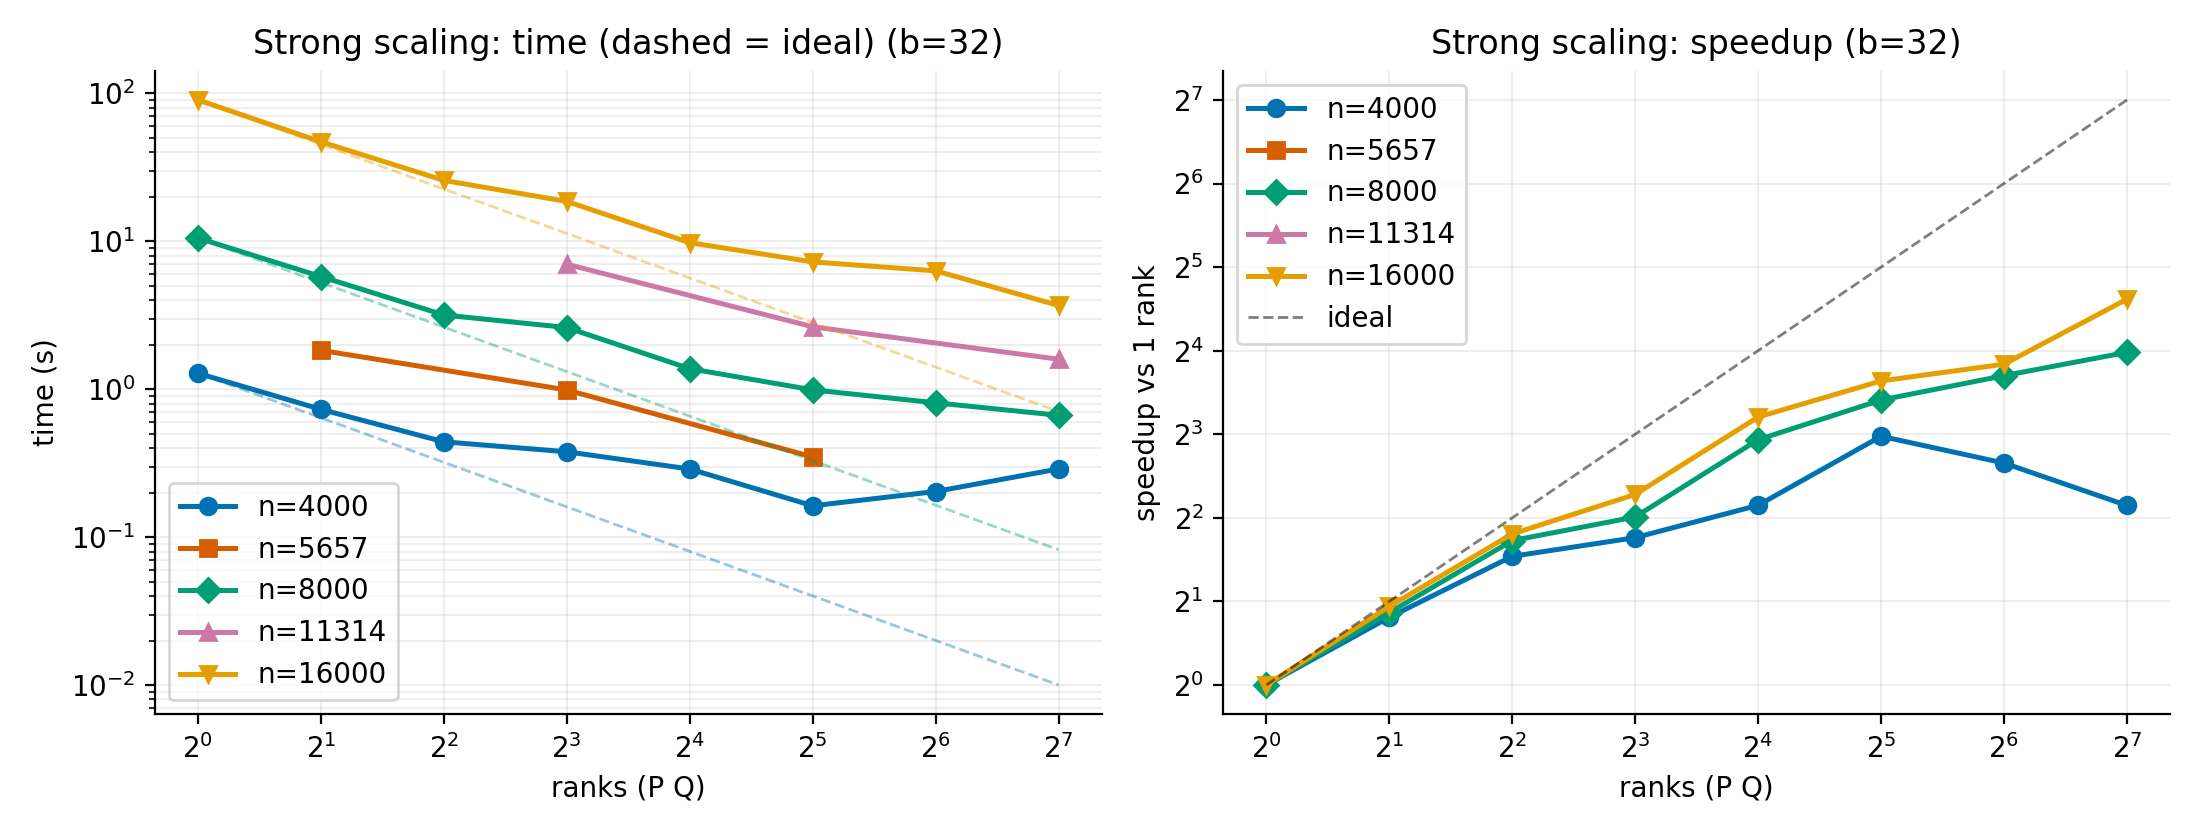
\includegraphics[width=0.92\textwidth]{figs/q2_strong_b32.png}
        \caption{$b=32$}
        \label{fig:q2_strong_b32}
    \end{subfigure}

    \medskip
    \begin{subfigure}{\textwidth}
        \centering
        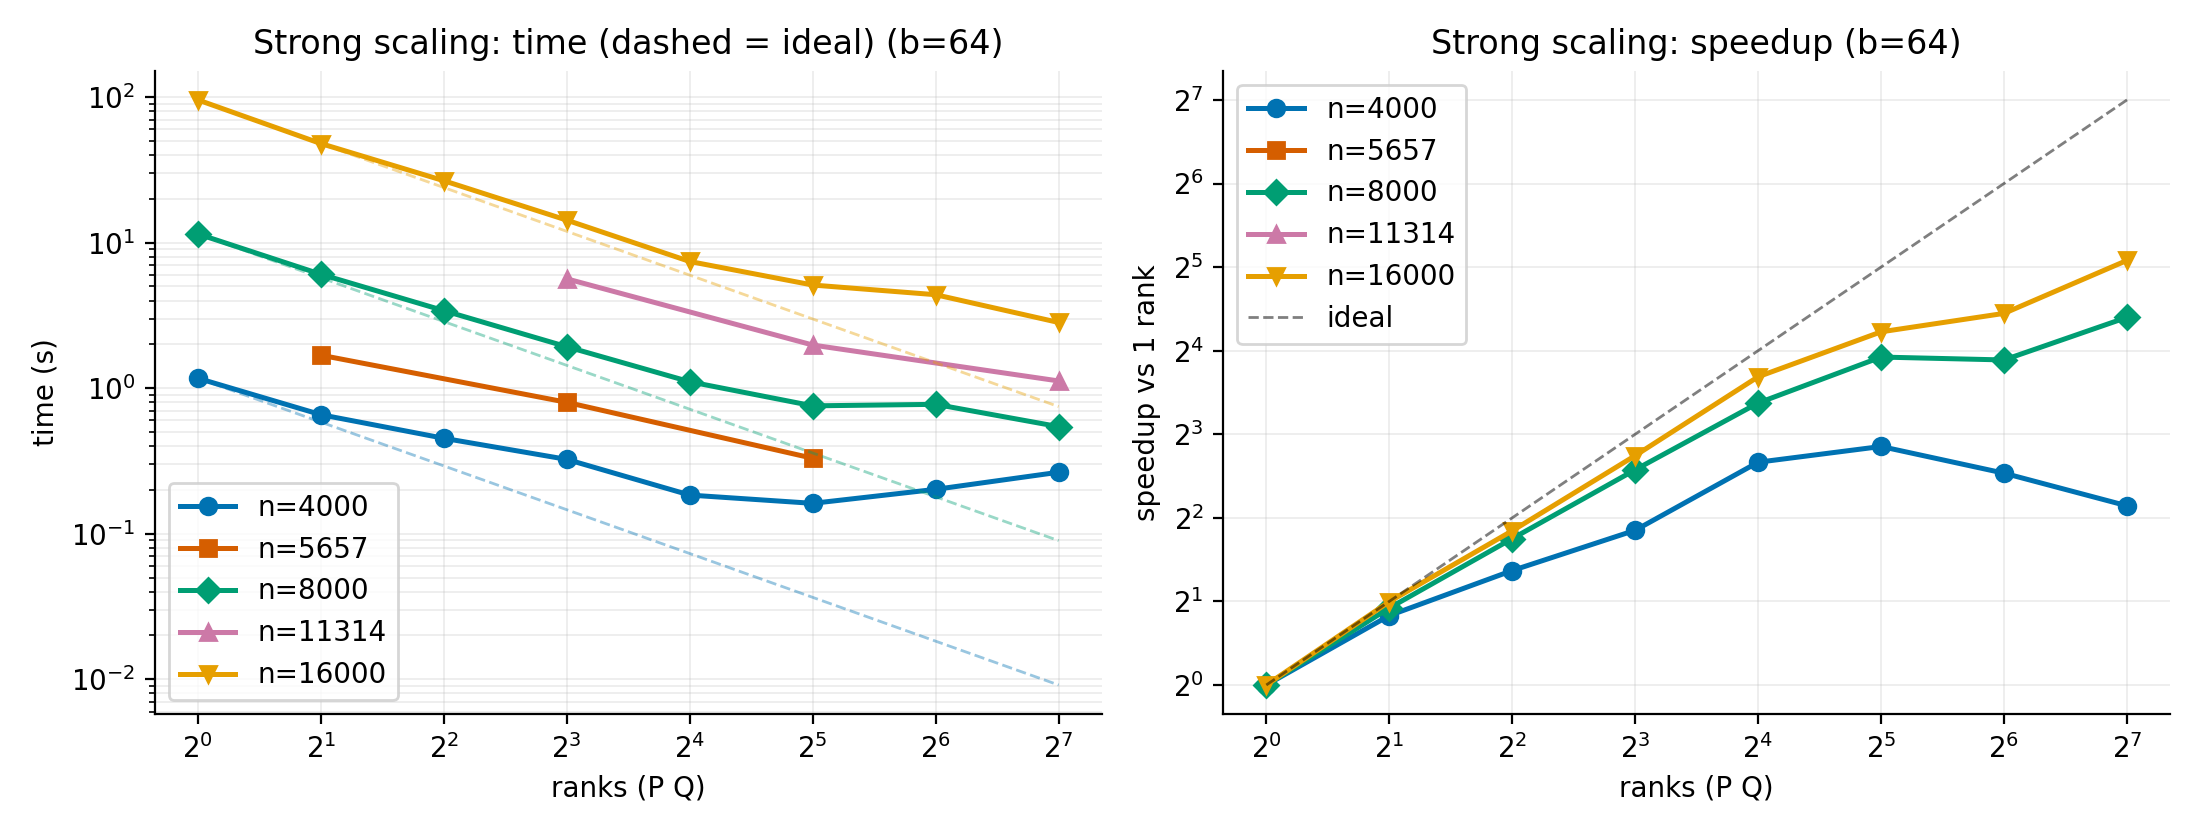
\includegraphics[width=0.92\textwidth]{figs/q2_strong_b64.png}
        \caption{$b=64$}
        \label{fig:q2_strong_b64}
    \end{subfigure}

    \medskip
    \begin{subfigure}{\textwidth}
        \centering
        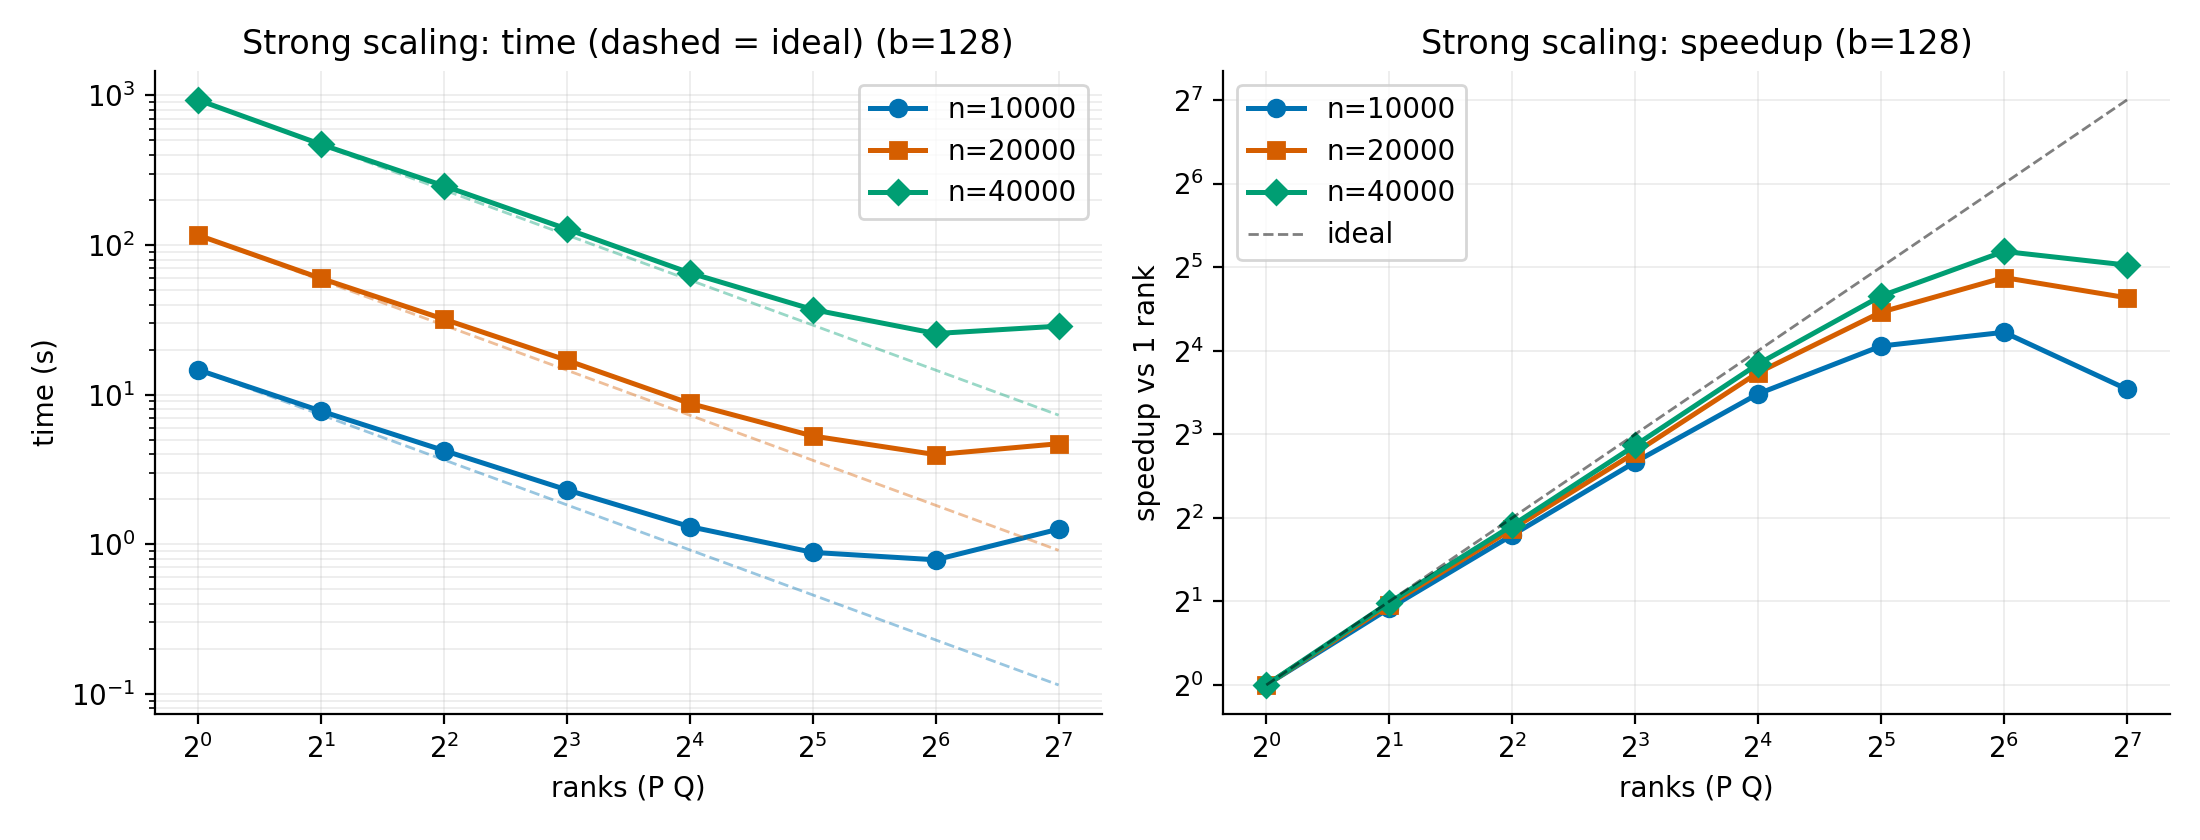
\includegraphics[width=0.92\textwidth]{figs/q2_strong_b128.png}
        \caption{$b=128$}
        \label{fig:q2_strong_b128}
    \end{subfigure}
    \caption{Q2 strong scaling for $n=10000$, $20000$ and $40000$ on 1 to 128 ranks, log--log, for block sizes $b=32$, $64$ and $128$. Left panels: time to factor; dashed lines are ideal $1/(PQ)$ scaling from the 1-rank run. Right panels: speedup over the 1-rank run; dashed line is ideal.}
    \label{fig:q2_strong}
\end{figure}

\begin{figure}[p]
    \centering
    \begin{subfigure}{\textwidth}
        \centering
        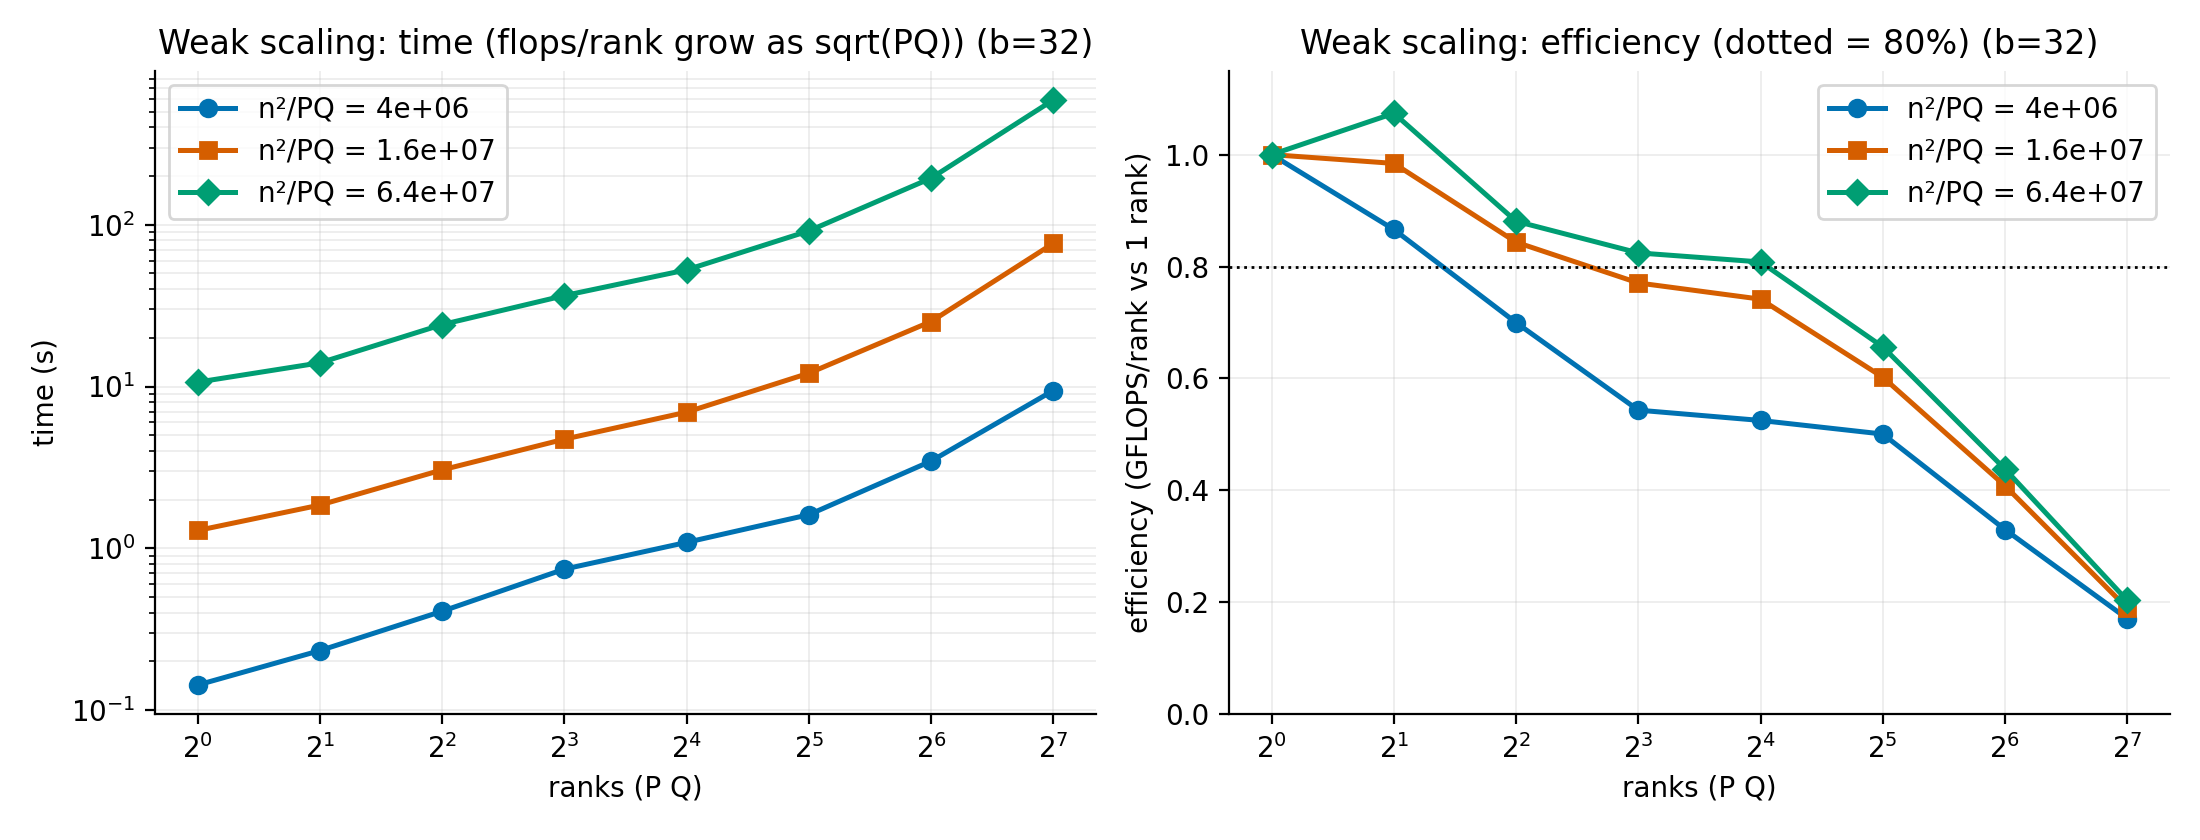
\includegraphics[width=0.92\textwidth]{figs/q2_weak_b32.png}
        \caption{$b=32$}
        \label{fig:q2_weak_b32}
    \end{subfigure}

    \medskip
    \begin{subfigure}{\textwidth}
        \centering
        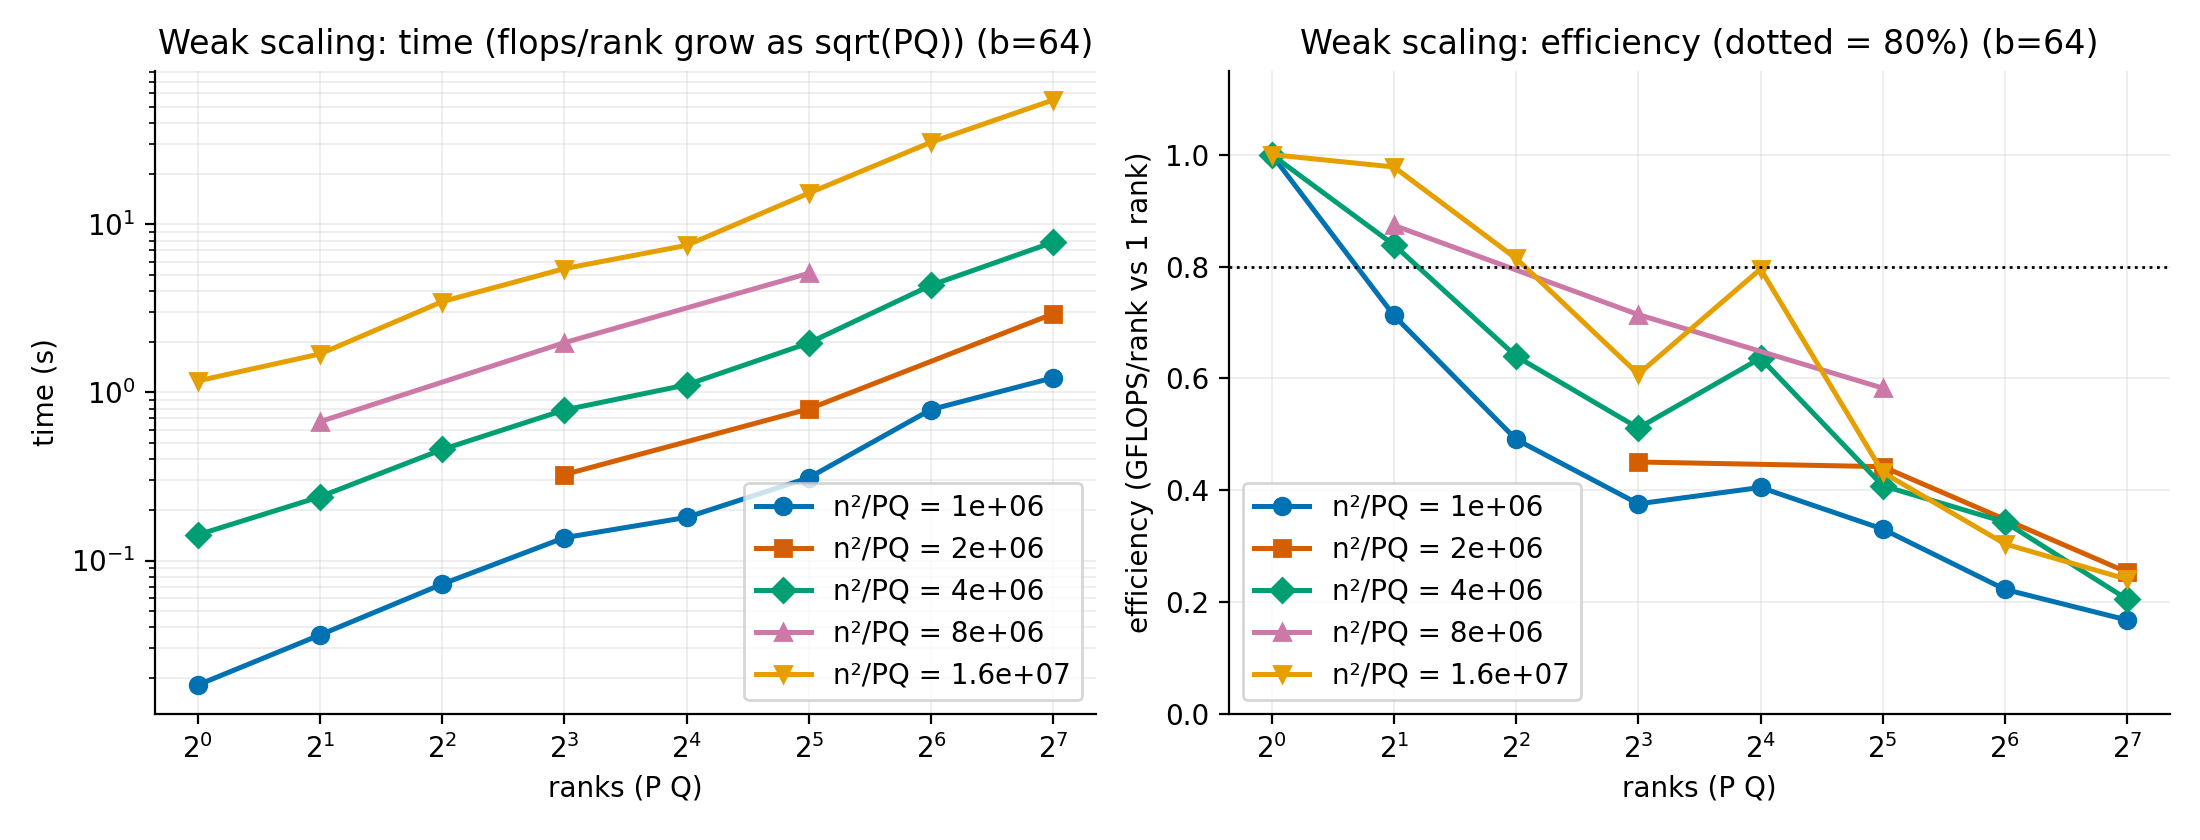
\includegraphics[width=0.92\textwidth]{figs/q2_weak_b64.png}
        \caption{$b=64$}
        \label{fig:q2_weak_b64}
    \end{subfigure}

    \medskip
    \begin{subfigure}{\textwidth}
        \centering
        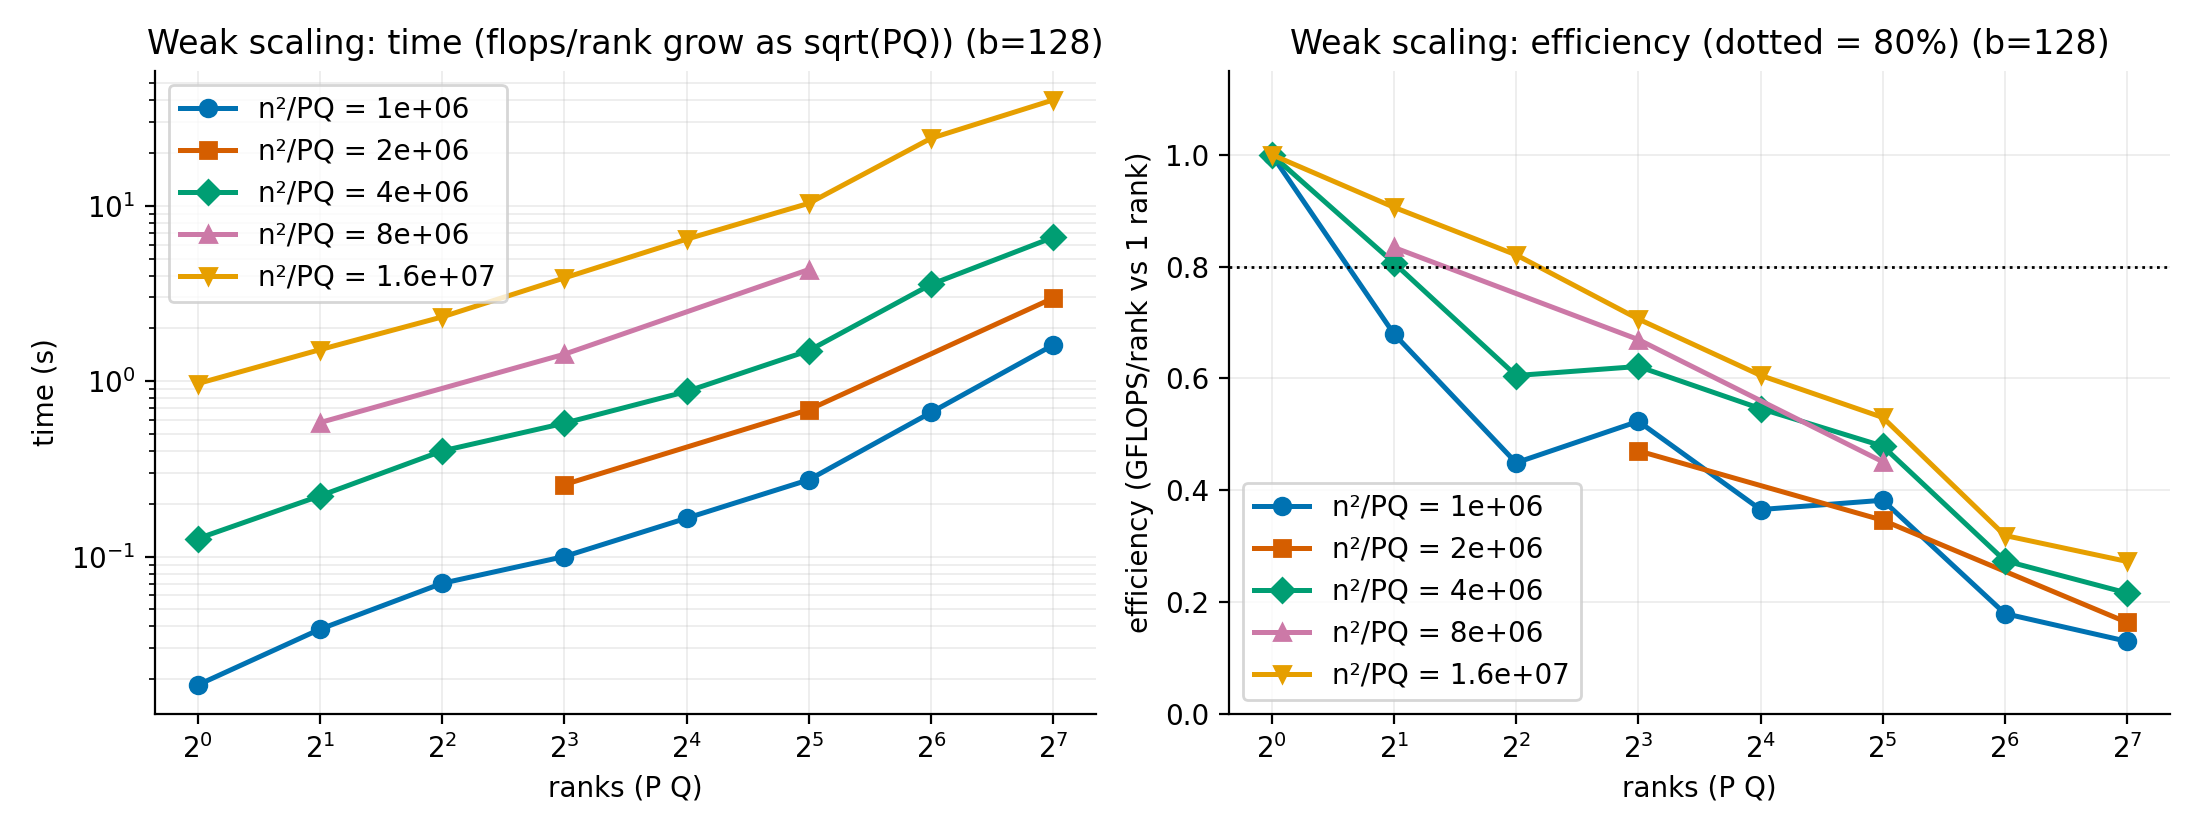
\includegraphics[width=0.92\textwidth]{figs/q2_weak_b128.png}
        \caption{$b=128$}
        \label{fig:q2_weak_b128}
    \end{subfigure}
    \caption{Q2 weak scaling for $n^2/(PQ)=4\times10^6$, $1.6\times10^7$ and $6.4\times10^7$ doubles per rank on 1 to 128 ranks, for block sizes $b=32$, $64$ and $128$. Left panels: time to factor (log scale). Right panels: efficiency, GFLOPS per rank divided by that of the 1-rank run with the same $b$ and $n^2/(PQ)$; dotted line is 80\%.}
    \label{fig:q2_weak}
\end{figure}

\FloatBarrier
\subsection{Local memory footprint for 80\% efficiency}
We again look at the total memory footprint, this time taking in to account the different block sizes in \cref{fig:q2_eff}.
As in the last two parts we see that at $b=128$ most of runs hit 80\% parallel efficiency for some local footprint tested.
This was not the case in the unblocked version, or even in the $b = 32$ or $b = 64$. 
This confirms the hypothesis that with the BLAS3 version we are more efficient with the local memory. 

\begin{figure}[htbp]
    \centering
    \begin{subfigure}[t]{0.49\textwidth}
        \centering
        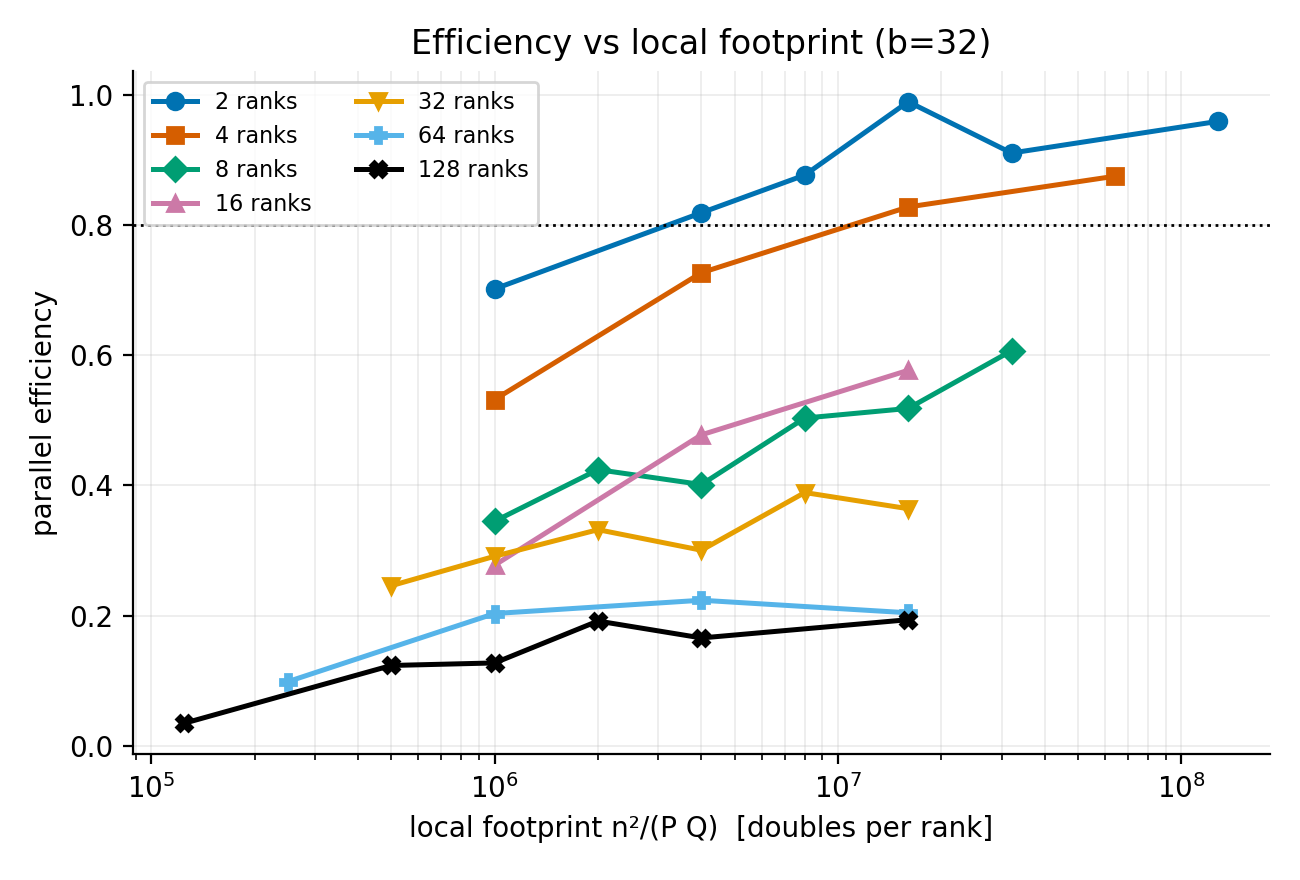
\includegraphics[width=\textwidth]{figs/q2_efficiency_footprint_b32.png}
        \caption{$b=32$ (best 1-rank: 37.4 GFLOPS)}
        \label{fig:q2_eff_b32}
    \end{subfigure}\hfill
    \begin{subfigure}[t]{0.49\textwidth}
        \centering
        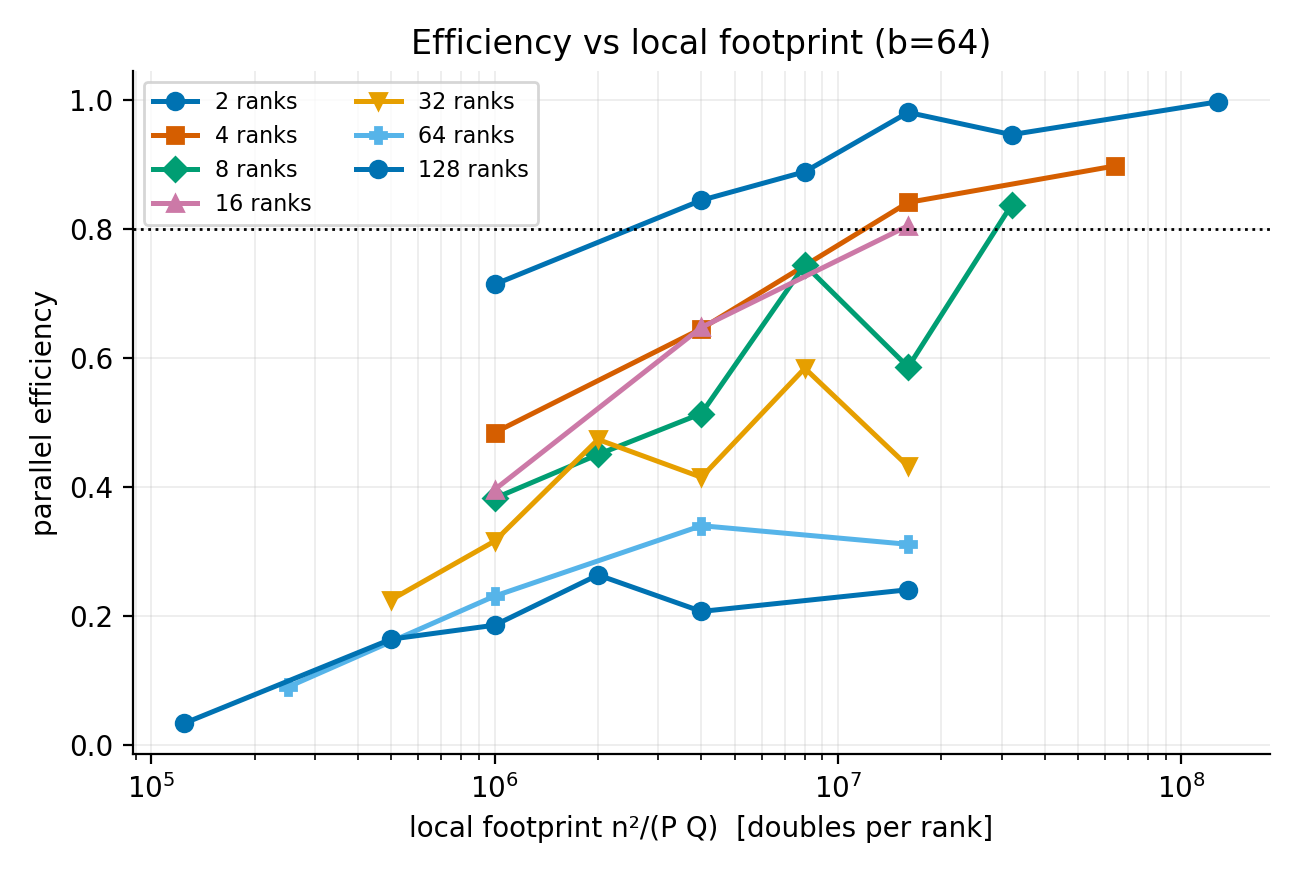
\includegraphics[width=\textwidth]{figs/q2_efficiency_footprint_b64.png}
        \caption{$b=64$ (best 1-rank: 41.0 GFLOPS)}
        \label{fig:q2_eff_b64}
    \end{subfigure}

    \medskip
    \begin{subfigure}[t]{0.49\textwidth}
        \centering
        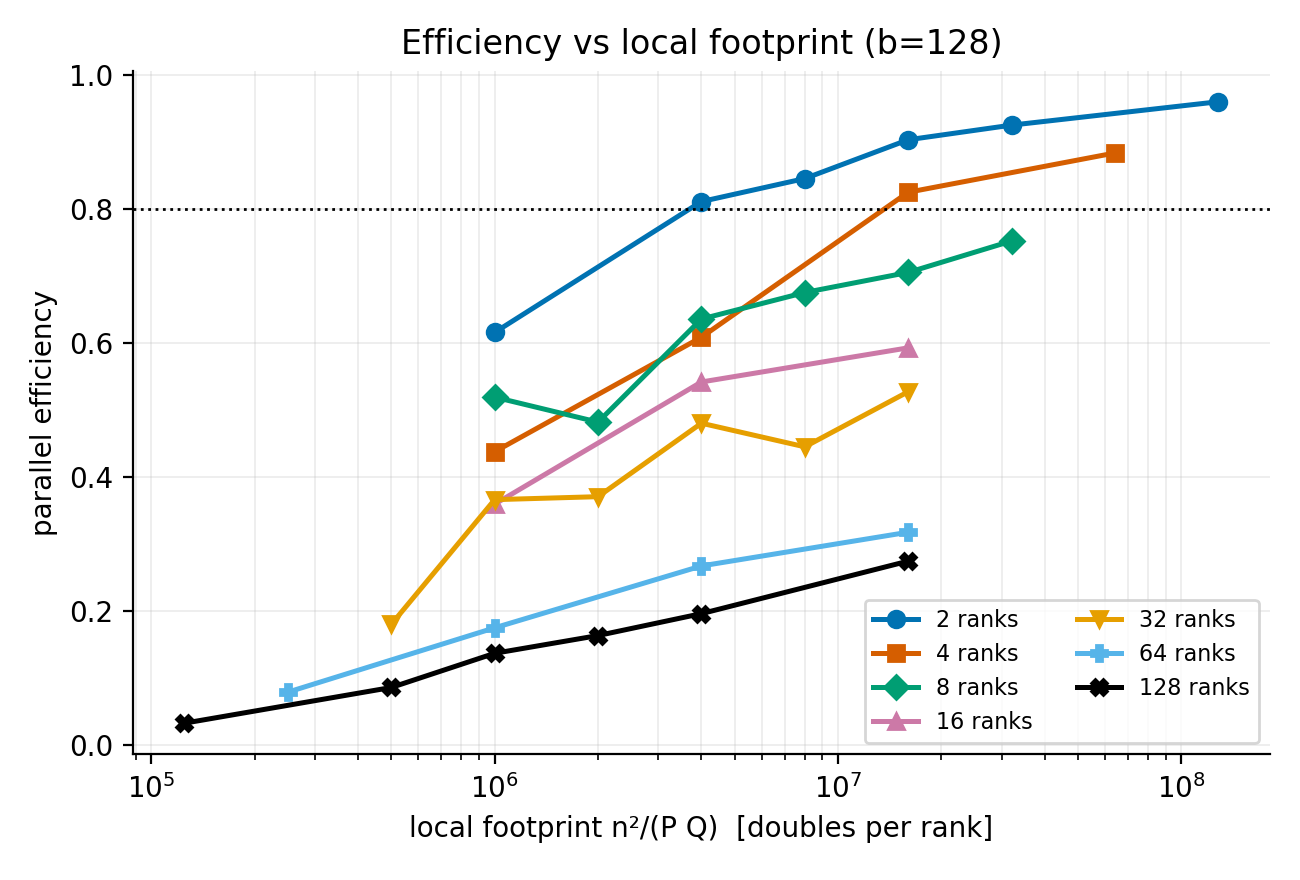
\includegraphics[width=\textwidth]{figs/q2_efficiency_footprint_b128.png}
        \caption{$b=128$ (best 1-rank: 45.8 GFLOPS)}
        \label{fig:q2_eff_b128}
    \end{subfigure}
    \caption{Q2 efficiency against the local footprint $n^2/(PQ)$ (doubles per rank) for $b=32$, $64$ and $128$, one curve per rank count, from every strong-scaling, weak-scaling and block-size-sweep run with more than one rank. Efficiency is GFLOPS per rank divided by the best 1-rank GFLOPS for that $b$. Dotted line: 80\%.}
    \label{fig:q2_eff}
\end{figure}

\FloatBarrier
\subsection{Observed GFLOPS}
In \cref{fig:q2_gflops} we see that we get many times more GFLOPS in the blocked case compared to the unblocked case, getting near or above $1000$ for all $b$ tried.
This makes sense as the BLAS3 nature alows the processor to spend more time on FLOPS and less on memory accesses.
We also see an increase in peak GFLOPS as $b$ increases with the runs at $b=32$ being around half as large as $b=128$.

\begin{figure}[p]
    \centering
    \begin{subfigure}{\textwidth}
        \centering
        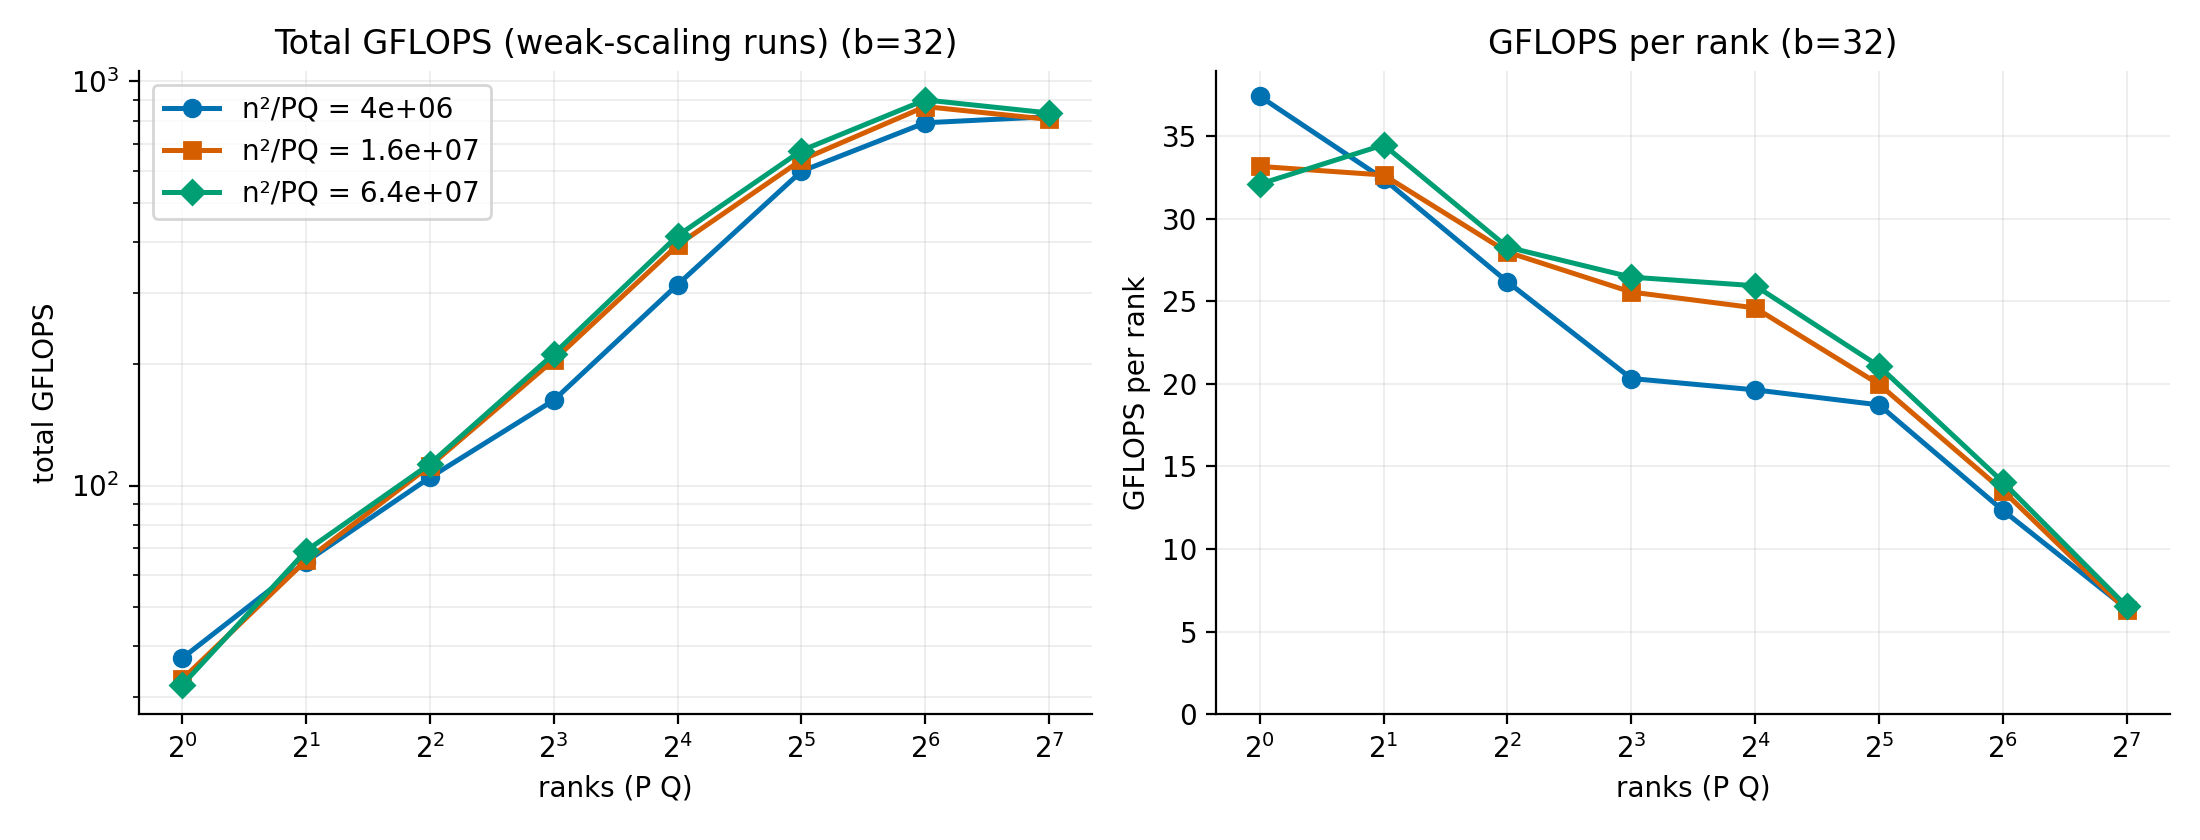
\includegraphics[width=0.92\textwidth]{figs/q2_gflops_b32.png}
        \caption{$b=32$}
        \label{fig:q2_gflops_b32}
    \end{subfigure}

    \medskip
    \begin{subfigure}{\textwidth}
        \centering
        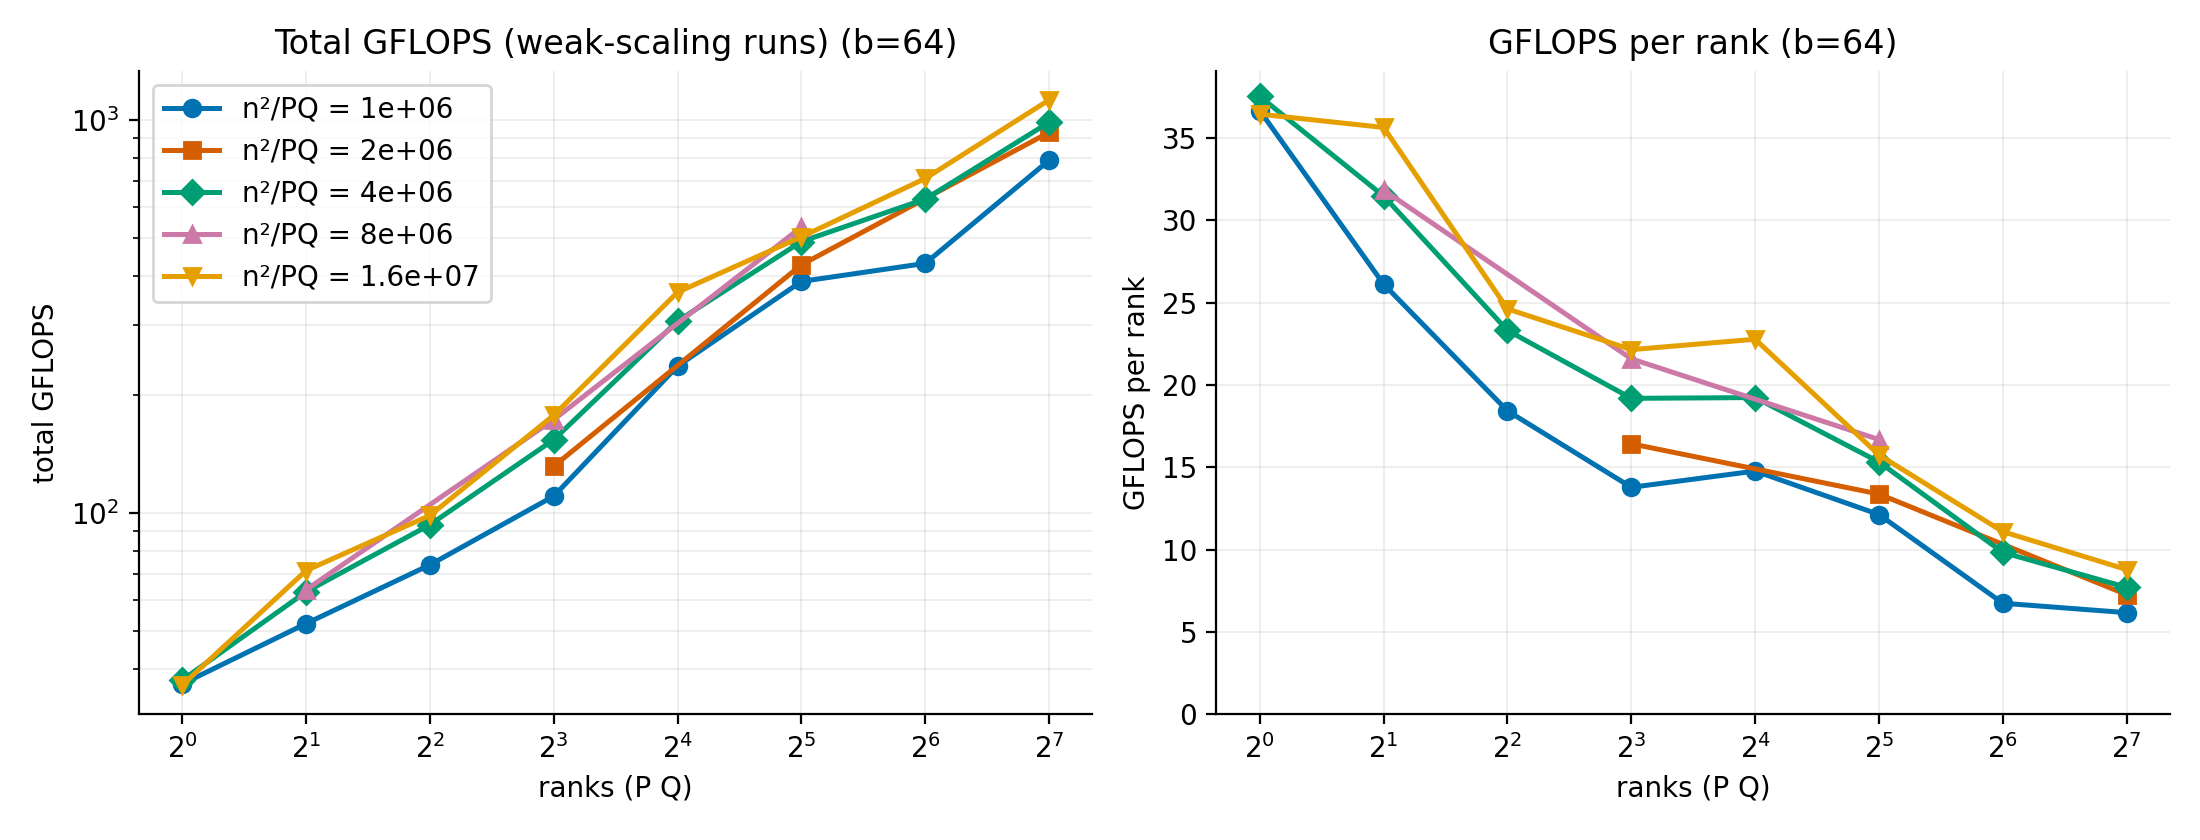
\includegraphics[width=0.92\textwidth]{figs/q2_gflops_b64.png}
        \caption{$b=64$}
        \label{fig:q2_gflops_b64}
    \end{subfigure}

    \medskip
    \begin{subfigure}{\textwidth}
        \centering
        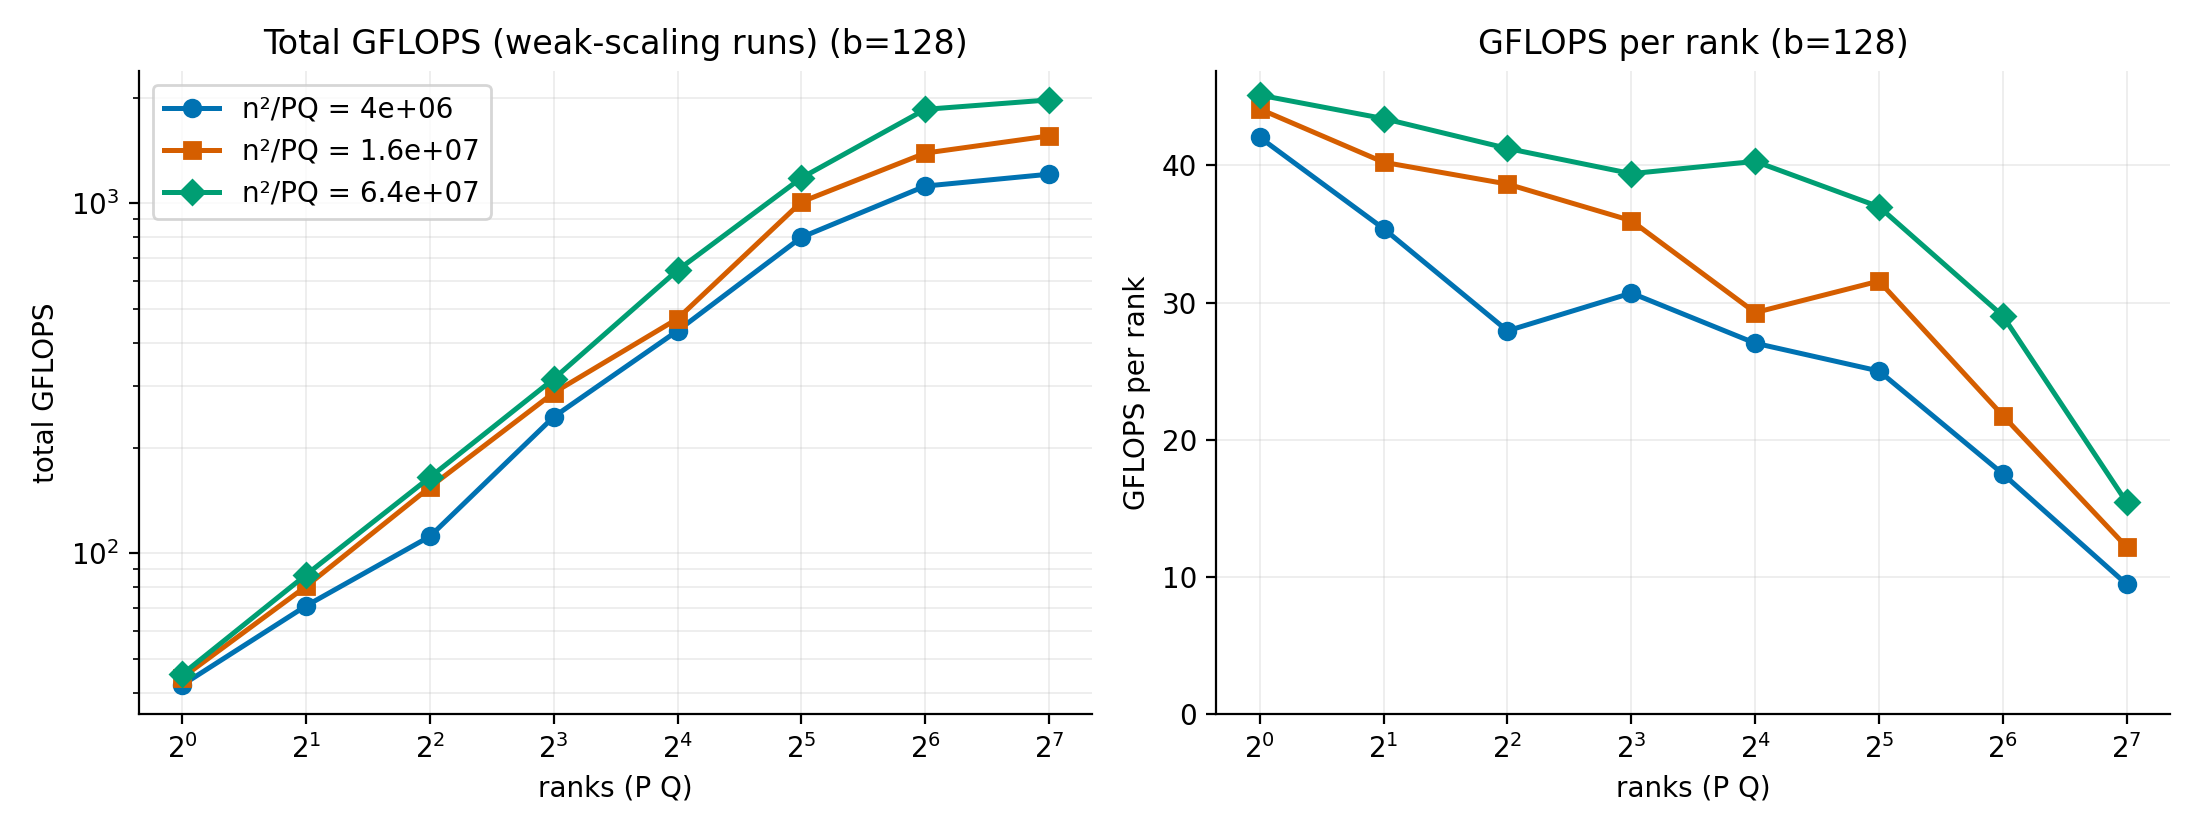
\includegraphics[width=0.92\textwidth]{figs/q2_gflops_b128.png}
        \caption{$b=128$}
        \label{fig:q2_gflops_b128}
    \end{subfigure}
    \caption{Q2 GFLOPS of the weak-scaling runs against the number of ranks for $b=32$, $64$ and $128$, one curve per $n^2/(PQ)$. Left panels: total GFLOPS (log scale). Right panels: GFLOPS per rank.}
    \label{fig:q2_gflops}
\end{figure}

\FloatBarrier
\subsection{Optimal block size}
Looking for the optimal block size, we see that in every case bigger $b$ is better though the results get noisier as $b$ gets larger.
The homework doc suggests looking up to 128 but it is likely a truely optimal block size lies a bit higher than that. 
Notable for higher rank runs, the GFLOPS per rank in \cref{fig:q2_bsweep} are less sensitive to block size.

\begin{figure}[!htbp]
    \centering
    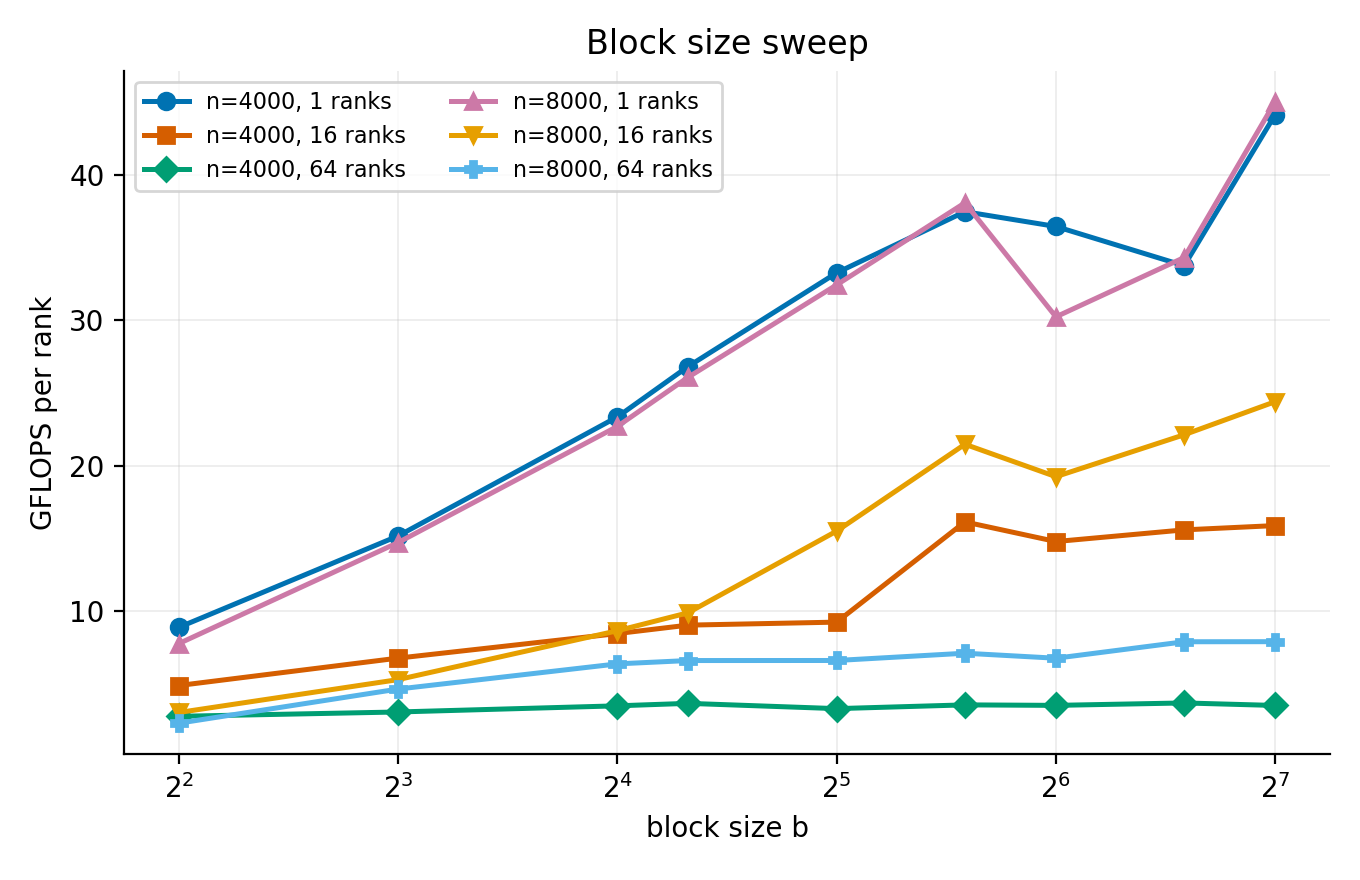
\includegraphics[width=0.75\textwidth]{figs/q2_bsweep.png}
    \caption{Block size sweep: GFLOPS per rank against $b=4$, $8$, $16$, $20$, $32$, $48$, $64$, $96$ and $128$ (log scale) for $n=4000$ and $n=8000$ on 1, 16 and 64 ranks.}
    \label{fig:q2_bsweep}
\end{figure}

\begin{figure}[!htbp]
    \centering
    \begin{subfigure}[t]{0.32\textwidth}
        \centering
        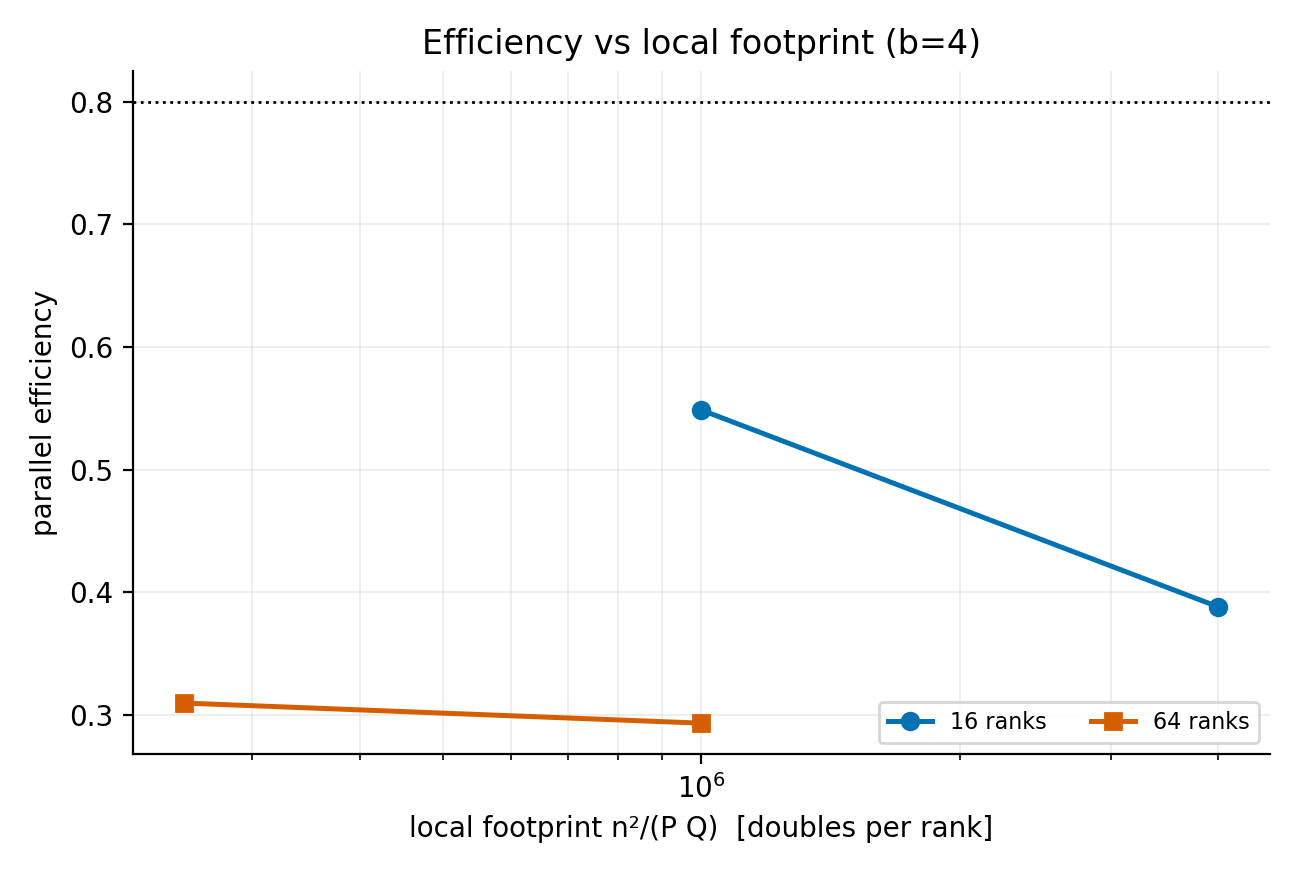
\includegraphics[width=\textwidth]{figs/q2_efficiency_footprint_b4.png}
        \caption{$b=4$}
        \label{fig:q2_eff_b4}
    \end{subfigure}\hfill
    \begin{subfigure}[t]{0.32\textwidth}
        \centering
        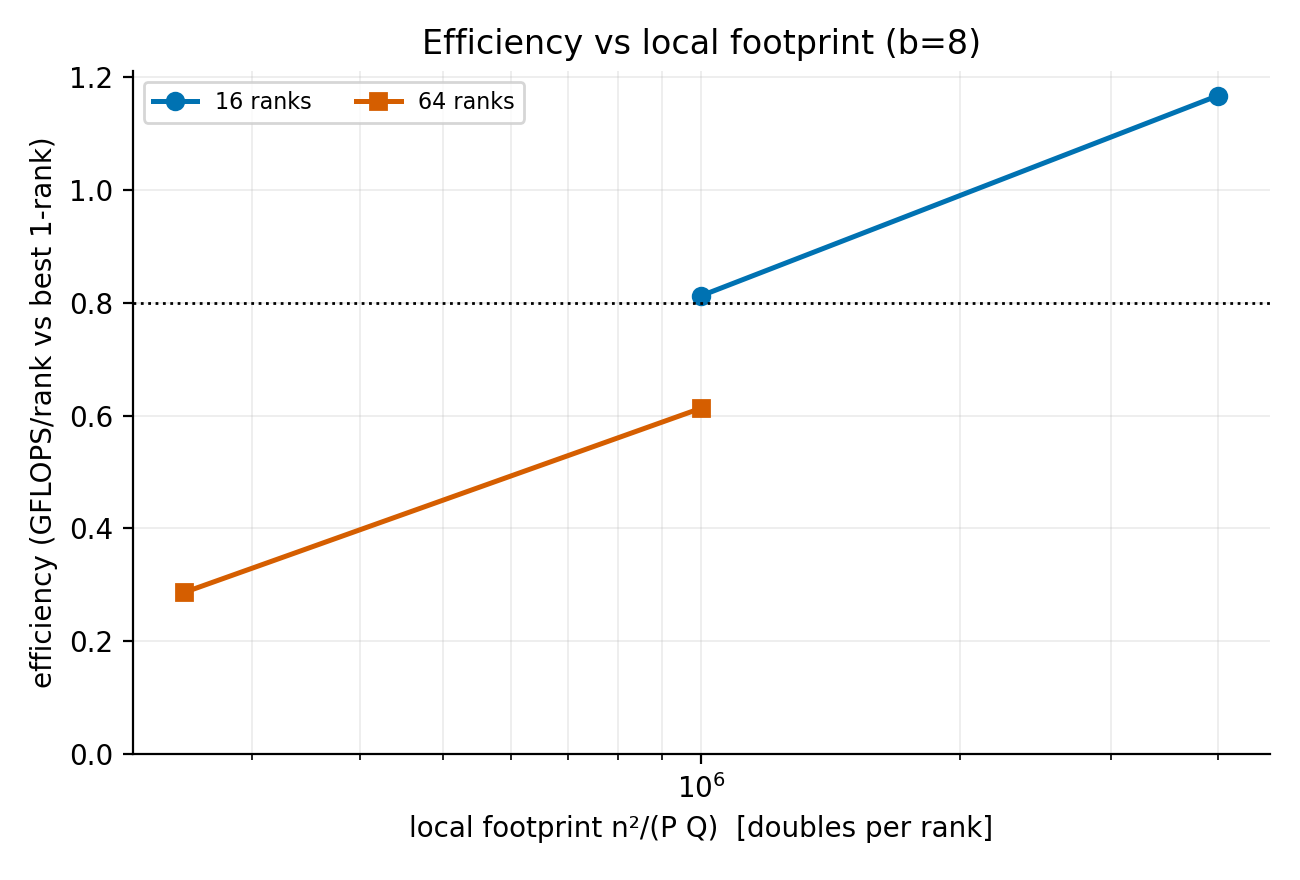
\includegraphics[width=\textwidth]{figs/q2_efficiency_footprint_b8.png}
        \caption{$b=8$}
        \label{fig:q2_eff_b8}
    \end{subfigure}\hfill
    \begin{subfigure}[t]{0.32\textwidth}
        \centering
        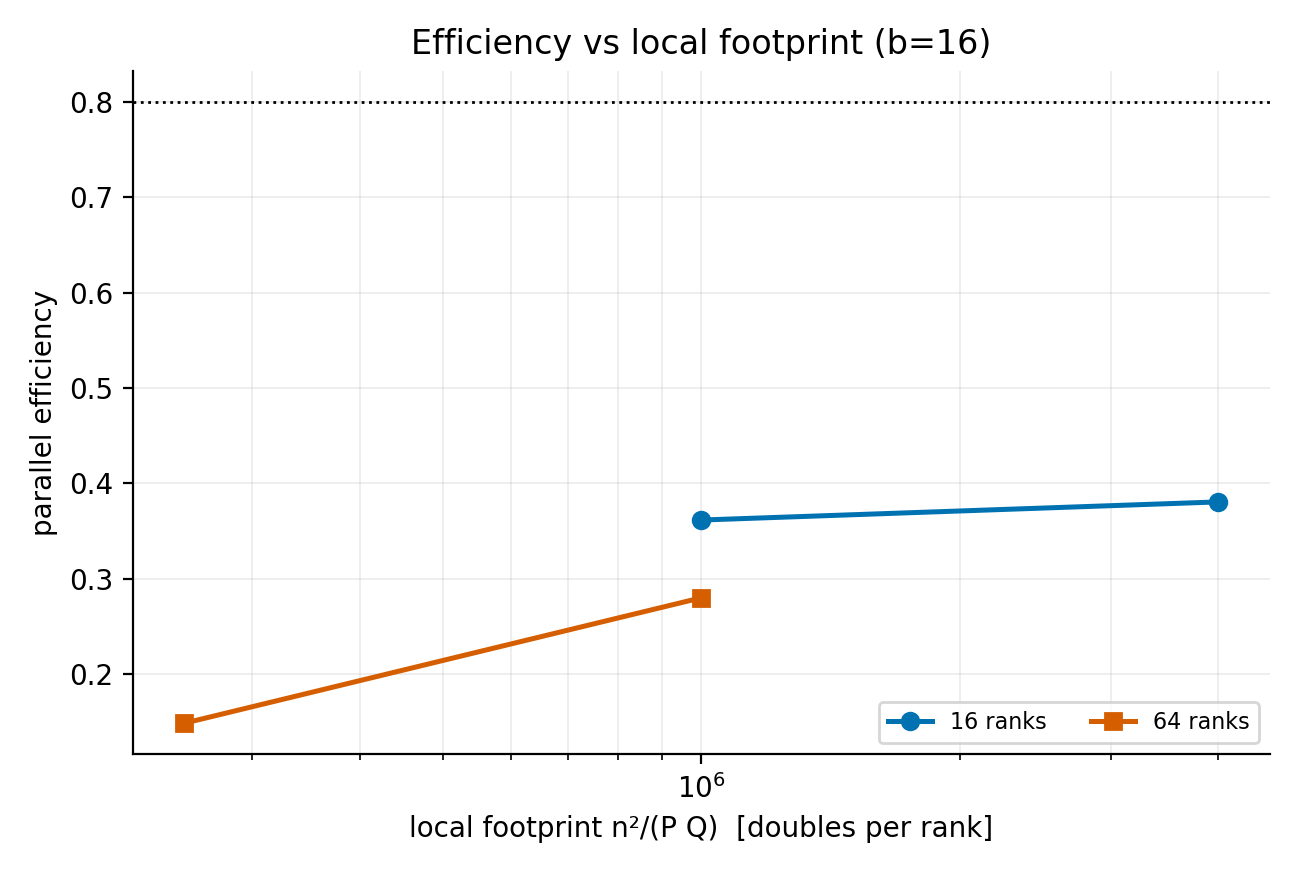
\includegraphics[width=\textwidth]{figs/q2_efficiency_footprint_b16.png}
        \caption{$b=16$}
        \label{fig:q2_eff_b16}
    \end{subfigure}

    \medskip
    \begin{subfigure}[t]{0.32\textwidth}
        \centering
        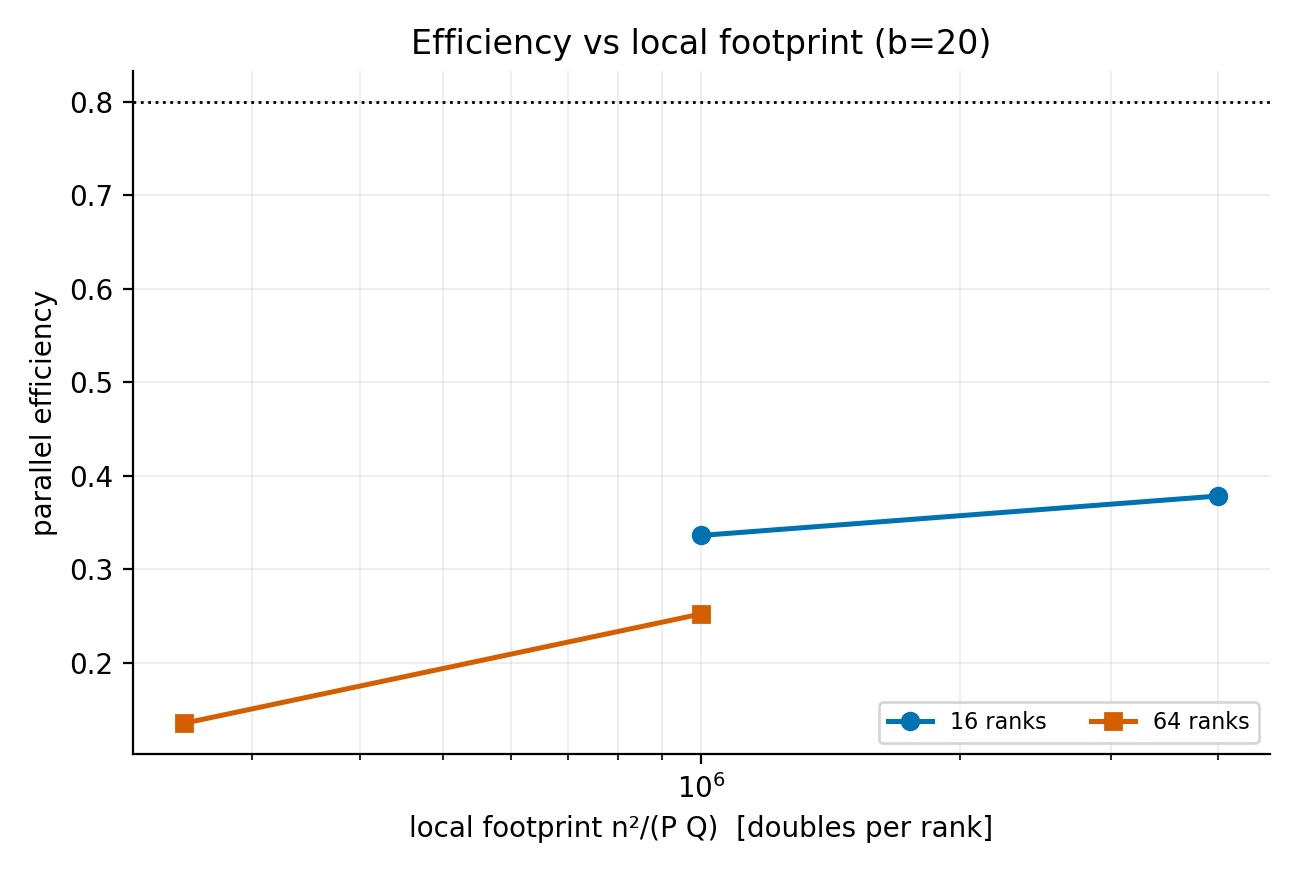
\includegraphics[width=\textwidth]{figs/q2_efficiency_footprint_b20.png}
        \caption{$b=20$}
        \label{fig:q2_eff_b20}
    \end{subfigure}\hfill
    \begin{subfigure}[t]{0.32\textwidth}
        \centering
        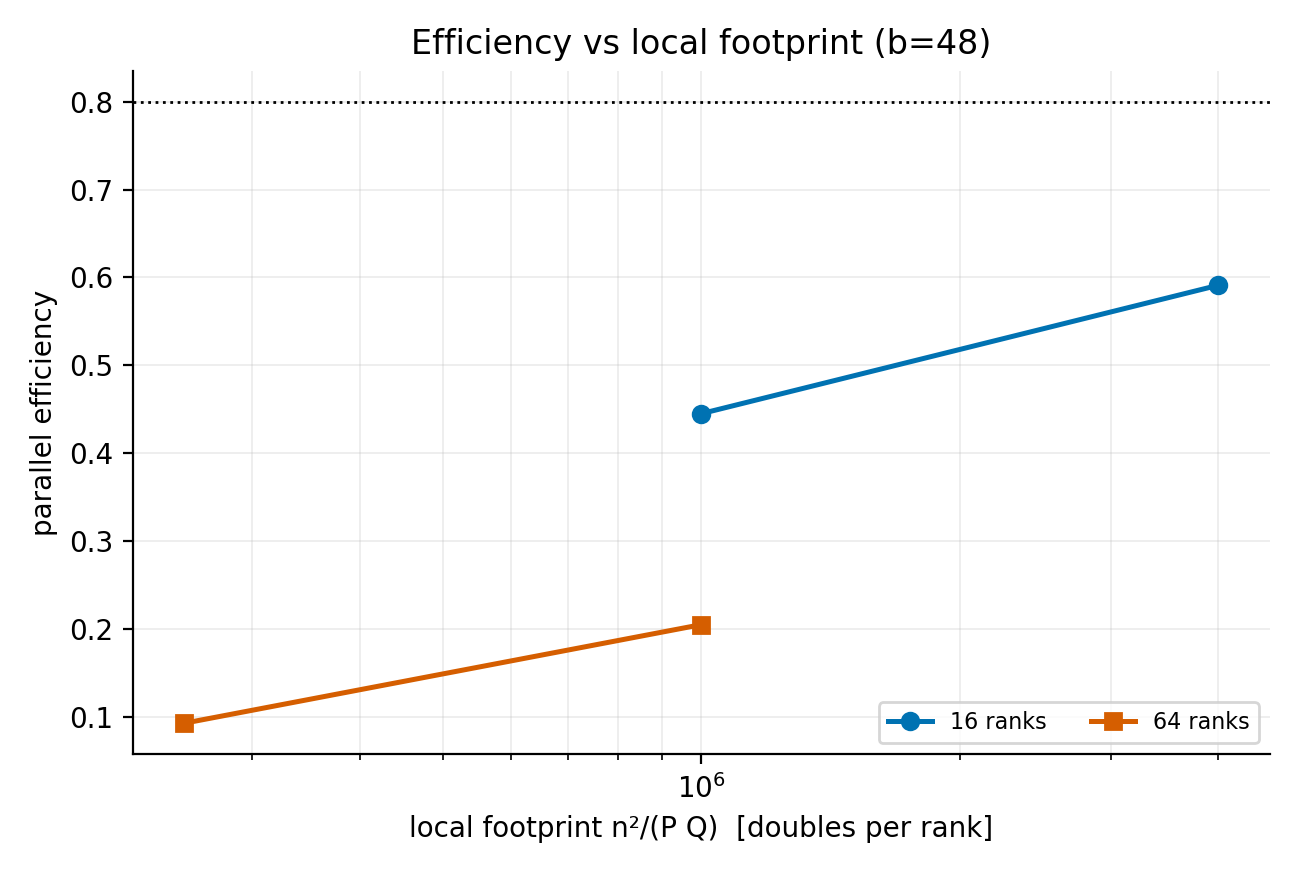
\includegraphics[width=\textwidth]{figs/q2_efficiency_footprint_b48.png}
        \caption{$b=48$}
        \label{fig:q2_eff_b48}
    \end{subfigure}\hfill
    \begin{subfigure}[t]{0.32\textwidth}
        \centering
        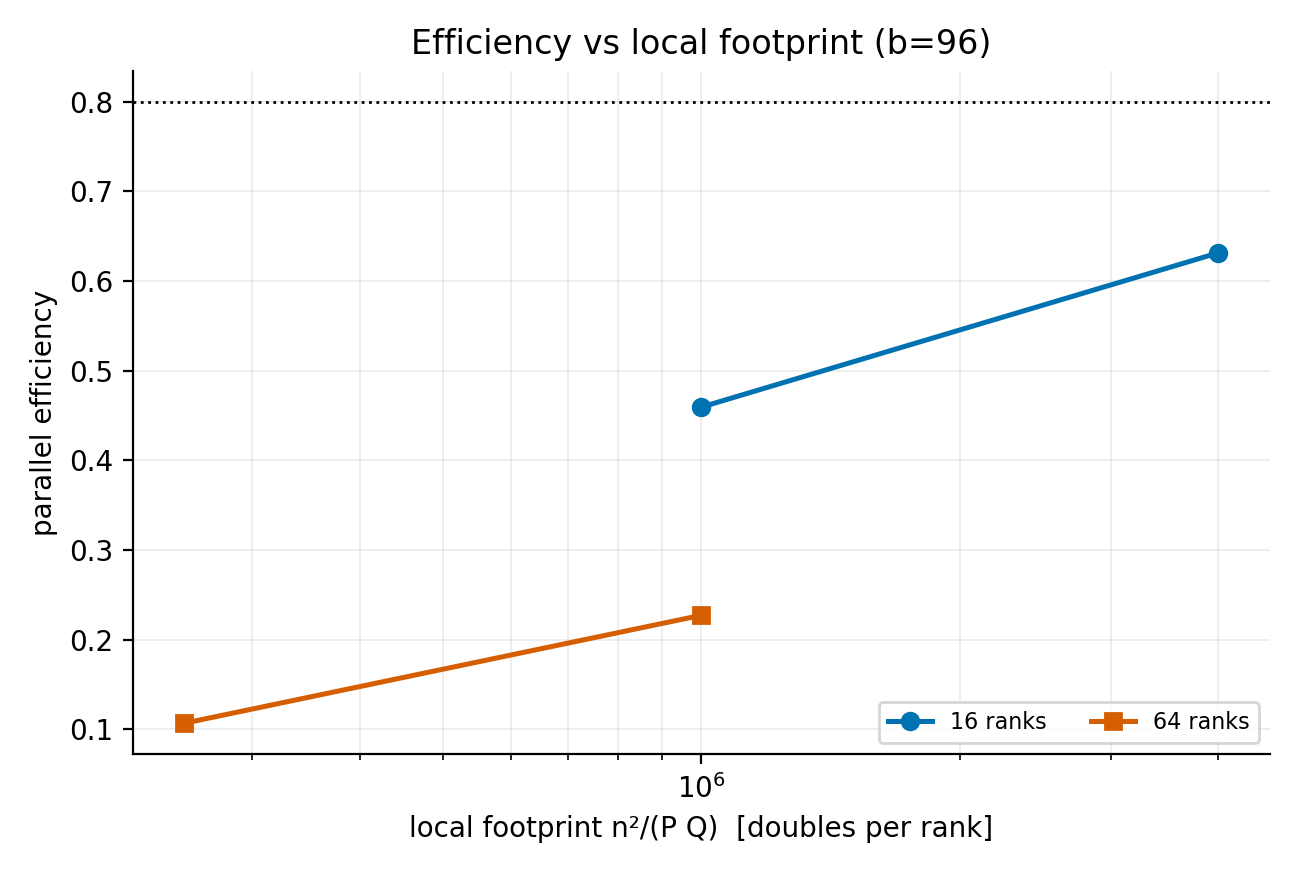
\includegraphics[width=\textwidth]{figs/q2_efficiency_footprint_b96.png}
        \caption{$b=96$}
        \label{fig:q2_eff_b96}
    \end{subfigure}
    \caption{Efficiency against the local footprint $n^2/(PQ)$ for the block sizes run only in the block size sweep ($n=4000$ and $8000$ on 16 and 64 ranks). Efficiency is GFLOPS per rank divided by the best 1-rank GFLOPS for that $b$ in the sweep. Dotted line: 80\%.}
    \label{fig:q2_eff_sweep}
\end{figure}

\end{document}
